%%%%%%%%%%%%%%%%%%%%%%%%%%%%%%%%%%%%%
%%%%% This example document / template has been created for      %%%%%
%%%%% use by the students of the MSc in Statistics of Imperial  	 %%%%%
%%%%% College London by Paul Ginzberg on 04 Aug 2014		 %%%%%
%%%%%%%%%%%%%%%%%%%%%%%%%%%%%%%%%%%%%

%%% Set documentclass options.
\documentclass[11pt,a4,singlespacing,titlepagenumber=on]{scrreprt}
%%%obsolete starting points. (ignore)
%\documentclass[a4paper,12pt,singlespace,report]{memoir}
%\documentclass[a4,11pt,singlespace,MSc]{icldt}


%%%%%%%%%%%%%%%%%%%%%%%%%%%%%%%%%%%%%
%%%%%% Load required packages with options %%%%%%%%%%%%%%
%%%%%%%%%%%%%%%%%%%%%%%%%%%%%%%%%%%%%

\usepackage[latin1]{inputenc} % May or may not be needed.
\usepackage[UKenglish]{babel}

%%% American Mathematical Society packages
\usepackage{amsfonts}
\usepackage{amssymb}
\usepackage{amsmath}
\usepackage{amsthm}
\usepackage{amsbsy}
%\usepackage{bm} % Possibly a better alternative to amsbsy for making bold typeface math.

%%% Graphics packages
\usepackage{graphicx}
%\graphicspath{{figures/}} % Useful if you have lots of images and want to keep thinks tidy by having a subfolder for images
%\usepackage{epstopdf} % If you produce your graphs as .eps files but then want to compile straight to PDF (e.g. because you are using TeXworks.) you may want to use this option. A better alternative of course would be to save all your graphs as *.pdf files from the start. Note that if you are compiling to pdf through PS/DVI then all your figures should be *.eps files and the epstopdf package should not be used.
%\usepackage{tikz} %For creating vector-graphics diagrams etc directly in LaTeX (takes some time to learn)
\usepackage[absolute]{textpos} % Used to position the Imperial College logo. You can comment this line and the next line out if you don't use the logo.
%\setlength{\TPHorizModule}{\paperwidth}\setlength{\TPVertModule}{\paperheight}
%\setlength{\TPHorizModule}{1cm}\setlength{\TPVertModule}{1cm}


%%% Referencing and cross-referencing
%\usepackage{color}
%\usepackage[colorlinks=false,linkcolor=red,urlcolor=cyan,citecolor=blue,breaklinks,plainpages=false,pdfpagelabels]{hyperref} % To make the hyperlinked cross-referencing visible.
\usepackage[colorlinks=false,pdfborder={0 0 0},plainpages=false,pdfpagelabels]{hyperref} % If you click on an item in the table of contents or a referenced equation/figure number, the PDF will go to the desired page. Neat isn't it?
% \usepackage[round,authoryear,sort]{natbib} % Enable bibtex-based bibliography generation
\usepackage{cite}
%\usepackage[square,numbers,sort&compress]{natbib} % If you want numbered referencing instead of author-year style.



%%%%%%%%%%%%%%%%%%%%%%%%%%%%%%%%%%%%%
%%%%% Create or control Macros   %%%%%%%%%%%%%%%%%%%%
%%%%%%%%%%%%%%%%%%%%%%%%%%%%%%%%%%%%%

%\setcounter{secnumdepth}{3} %If you want subsubsections to be numbered
\numberwithin{equation}{chapter} % Reset equation numbers after each chapter.

%%% Theorem environments
\newtheorem{theorem}{Theorem}%[chapter]
\newtheorem{proposition}[theorem]{Proposition}%[chapter]
\newtheorem{definition}[theorem]{Definition}%[chapter]
\newtheorem{lemma}[theorem]{Lemma}%[chapter]
\newtheorem{corollary}[theorem]{Corollary}%[chapter]
%
\theoremstyle{remark}
\newtheorem{remark}[theorem]{Remark}%[chapter]
\newtheorem{example}[theorem]{Example}%[chapter]

%%% Potentially useful style changes:
%\renewcommand{\titlefont}{\normalcolor \normalfont \bfseries} %Change the title font from sans-serif to serif (the same font used for the rest of the document).
%\renewcommand*{\labelitemi}{$\bullet$} %Bullet points in the itemize environment.
%\renewcommand*{\tilde}{\widetilde} % Wider tildes
%\renewcommand*{\bar}{\overline} % Wider conjugate bars

%%% Examples of commands/macros that could be useful:
%\newcommand{\expectation}[1]{\mathbb{E}\left[ #1 \right]}
%\newcommand*{\setR}{{\mathbb R}}
%\newcommand{\commentify}[1]{} %Gives you an alternative way (other than %) to comment things out.
%%% These commands make it faster to get the correct roman font in equations: (similar to \exp, \cos, \sin etc). Alternatively yuo can always use e.g. $\mathrm{Var}$
%\DeclareMathOperator{\bigo}{O}
%\DeclareMathOperator{\littleo}{o}
%\DeclareMathOperator{\var}{Var}
%\DeclareMathOperator{\cov}{Cov}
%\DeclareMathOperator{\trace}{trace}
%\DeclareMathOperator{\sign}{sgn}
%\DeclareMathOperator{\rank}{rank}
%\DeclareMathOperator{\vecrm}{vec} % The \vec command already exists.




%%%%%%%%%%%%%%%%%%%%%%%%%%%%%%%%%%%%%
%%%%% Define how to create the title page  %%%%%%%%%%%%%%%%
%%%%%%%%%%%%%%%%%%%%%%%%%%%%%%%%%%%%%
\makeatletter
\newcommand*{\supervisor}[1]{\gdef\@supervisor{#1}}
\newcommand*{\CID}[1]{\gdef\@CID{#1}}
\newcommand*{\logoimg}[1]{\gdef\@logoimg{#1}}
\renewcommand{\maketitle}{
\begin{titlepage}
\ifdefined\@logoimg
\begin{textblock*}{8cm}(1.75cm,1.75cm)
\includegraphics[width=70mm]{\@logoimg}
\end{textblock*}
\vspace*{1cm}
\else
%\vspace*{0cm}
\fi
\begin{center}
\vspace*{\stretch{0.1}}
Imperial College London\\
Department of Mathematics\par
\vspace*{\stretch{1}} % This inserts vertical space and allows you to specify a relative size for the vertical spaces.
{\titlefont\Huge \@title\par} % If your title is long, you may wish to use \huge instead of \Huge.
\vspace*{\stretch{2}}
{\Large \@author \par}
\vspace*{1em}
{\large CID: \@CID \par}
\vspace*{\stretch{0.5}}
{\large Supervised by \@supervisor \par}
\vspace*{\stretch{3}}
{\Large \@date \par}
\vspace*{\stretch{1}}
{\large Submitted in partial fulfilment of the requirements for the
MSc in Statistics of Imperial College London}
\vspace*{\stretch{0.1}}
\end{center}%
\end{titlepage}%
}
\makeatother

%%% And the plagiarism declaration
\newcommand*{\declaration}{%
\vspace*{0.3\textheight}
The work contained in this thesis is my own work unless
otherwise stated.\\
\vspace*{0.1\textheight}\\
\hspace*{0.25\textwidth}Signed: \hspace{0.25\textwidth} Date:
\clearpage}

%%% And the abstract page
\renewenvironment{abstract}%
{\chapter*{Abstract}\thispagestyle{plain}}%
{\clearpage}
%%% And why not change the quote environment
\newenvironment{myquote}%
{\begin{quote}{\Large{}``}}%
{{\Large{}''}\end{quote}}




%%% Actual words used in the title page
\title{Adaptive learning for the restless bandit problem, with an application to online advertising}
\author{Alex Gillis}
\CID{00881910}
\supervisor{Supervisor Dr. Christoforos Anagnostopoulos}
\date{\today}
\logoimg{Imperial__4_colour_process.jpg} %The filename for the logo, if you want one. The logo file must be in the same directory as your *.tex file.

%%%%%%%%%%%%%%%%%%%%%%%%%%%%%%%%%%%%%
%%%%% End of preamble and start of document %%%%%%%%%%%%%%
%%%%%%%%%%%%%%%%%%%%%%%%%%%%%%%%%%%%%

\begin{document}


\maketitle %Generates the Title Page

\declaration %Insert plagiarism statement

\begin{abstract}

Our work formulates the Real Time Bidding problem as a multi-armed bandit.

We review current practises and argue that they are limited in their approach. 

We then provide a template for a more a principled approach where the domain is first modelled and then decision policies derived from this model. We demonstrate how significant performance improvements are possible and how the approach may be adapted to new scenarios.
 
In particular we develop a K-stage binomial model beating standard click-through-rate optimisation. We also draw attention to Thompson Sampling and Gittins Indices as techniques well suited to make use of custom binomial models.

\end{abstract}

\newpage
\chapter*{Acknowledgements}

I would like to express my appreciation to my supervisor, Dr Anagnostopoulos for his great generosity with his time, constructive feedback, enthusiastic guidance and being a pleasure to work with.

I would also like to thank Advance media for the exposure to the many practical dimensions of running online campaigns, as well as providing RTB campaign data. 

Finally, I wish to thank my wife for her incredible support throughout the project as well as her dedication to our four month old restless bandit, Daisy.

\newpage

% Automatically create a table of contents
\renewcommand{\contentsname}{Table of Contents}
\tableofcontents
\newpage

% Figure and table lists if you want them.
%\cleardoublepage
%\phantomsection
\listoffigures 
%\addcontentsline{toc}{chapter}{\listfigurename}
%\newpage
%\phantomsection
%\listoftables  
%\addcontentsline{toc}{chapter}{\listtablename}
%\newpage

\chapter{Introduction}

Our research formulates the real time bidding (RTB) problem as a multi-armed bandit (MAB). There are no papers addressing this directly, we therefore study RTB and MAB research separately. 

We first review current literature on RTB modelling. Current MAB approaches will be discussed separately in section 4. Research relating to binomial model fitting is discussed in section 3.


\section{Real Time Bidding}

An RTB campaign has a fixed budget and runs over the course of a number of months. The budget is spent bidding for \textbf{impressions}. If the bid is successful, an advert will be shown on the web page. If the user clicks on the ad, it will be recorded. A click is considered to be \textbf{converted} in to an \textbf{acquisition} if the user then performs the campaign's target action. Typically this would be to buy a product or sign up to a mailing list.

\begin{itemize}
	\item CTR (click-through-rate) - clicks per impression
	\item CVR (conversion rate) - acquisitions per click 
	\item AQR (acquisition rate) - acquisitions per impression
	\item CPA (cost per acquisition) - budget spent per acquisition
	\item CPC (cost per click) - budget spent per click
\end{itemize}

There are a several dimensions to the problem - estimating CTR rate for different placements, estimating acquisition rate and optimising bid level over course of campaign.

Richardson et al. ~\cite{Richardson:2007:PCE:1242572.1242643} discuss the benefits and limitations of a priori CTR prediction. Chen et al ~\cite{Chen:2011:RBA:2020408.2020604} and Ghosh et al. (Adaptive Bidding) ~\cite{Ghosh:2009:ABD:1526709.1526744} develop algorithms which optimise bid levels online. While Chen et al ~\cite{Chen:2011:RBA:2020408.2020604} focus on dynamic bid adjustment strategies to optimally meet campaign constraints, Ghosh et al. ~\cite{raey} look to 'learn' the bid distribution acknowledging the exploration-exploitation trade off, though not explicitly formulating as a MAB problem.

Li et al. ~\cite{Li:2010:CAP:1772690.1772758} explore the contextual multi armed bandit problem as applied to news article recommendation, while Yue ~\cite{yue2012hierarchical} and Pandey ~\cite{pandey2007bandits} use knowledge about the item and the arm inter-relatedness to speed convergence of the bandit arms.

\section{Our contribution}

No papers were found formulating the RTB as a MAB explicitly. Also, many practical aspects of the RTB problem have been overlooked - such as predicting acquisition rate, optimal explore-exploit trade offs for ad placement given time/budget limited campaigns. There also appears room to improve the combination of online and offline optimisation by treating our offline optimisation as a Bayesian prior to our online optimisation.

We also believe that much of the MAB applications literature has the following short comings:

\begin{enumerate}
	\item Development of 'one-size-fits-all decision algorithms' and heuristics, without principled ways to customise tools to specific problems.
	\item Over emphasis on asymptotic optimality and scalability overlooks poor performance on many common problems.
\end{enumerate}

We provide a template for a more a principled approach and demonstrate very substantial performance improvements. We demonstrate the importance of both:

\begin{enumerate}
	\item A well motivated custom model.
	\item A decision policy based on that model over generic exploration algorithms.
\end{enumerate}

There are a range of games where a generic model and asymptotic performance policies are inappropriate:

\begin{enumerate}
	\item Games with a low number of rounds, for example RTB platforms with batched feedback. The performance of these games are dominated by constant order terms, not asymptotic performance. Our later results provide examples of this. 
	\item Games with low information per round, for example, some RTB campaigns may only get one high-value acquisition for 1 million impressions. Here it is vital that our model leverage as much information as possible from other indicators.
	\item Non-stationary rewards (restless bandits), have rewards that drift or jump over time. Here we must learn the underlying reward quickly to exploit it before it changes. Our decision policy must also understand that exploration may have a lower value because the information can not be exploited for the entirety of the game.
\end{enumerate}

The common element in these games is the importance of extracting maximum information from each event. Figure 1.1 demonstrates the kind of performance improvement can be achieve through custom models and a model based decision policy.

\begin{figure}[p]
    \centering
    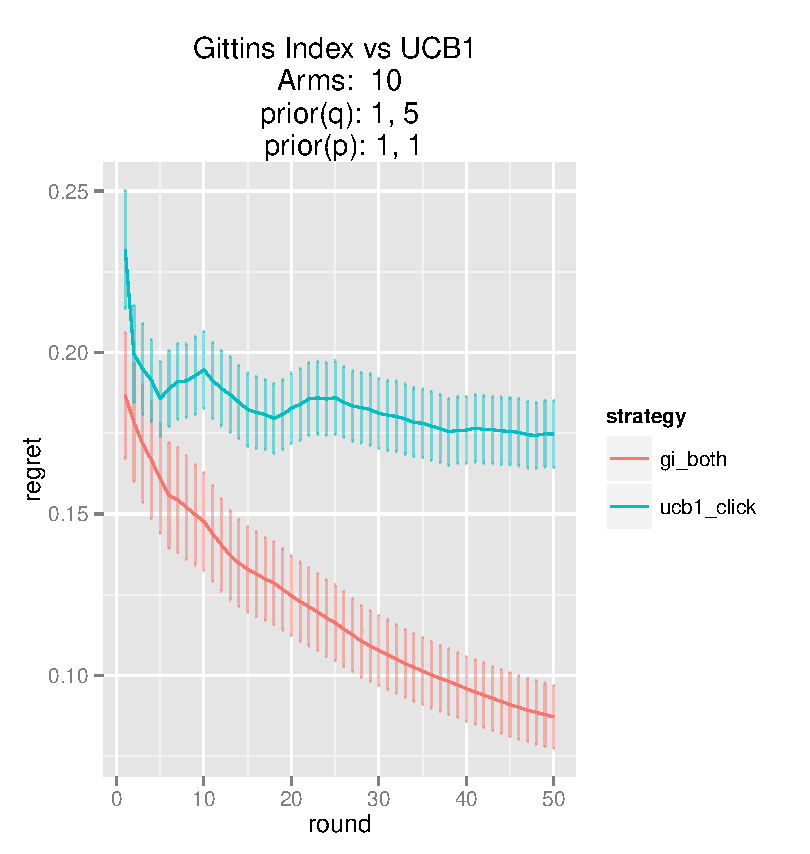
\includegraphics[scale=0.7]{GIvsUCB1.pdf}
    \caption{Mean regret of Gittins index strategy vs UCB1}
    \label{fig:GIvsUCB1}
\end{figure}


\section{Objective}
Our objective is to develop a model which minimises the cost per acquisition over the course of a campaign, whilst meeting budget constraints. We propose a number of innovations:
\begin{enumerate}
	\item A model to estimate CPA (as well as CPC).
	\item To elegantly address the trade off between offline and online estimation (discussed by Richardson) by offline generation of Bayesian prior for CTR.
	\item To model the E-E trade off as a MAB problem, putting a value on exploration for long and short campaigns.
	\item To incorporate the time and budget limitations in exploration of the MAB problem.
\end{enumerate}


\chapter{RTB Data}

The following data was provided by Advance media and represents a typical RTB campaign, though acquisition rates can be much lower.

We have 3 vector valued random variables. The ith index represents the values for site domain (website) i for a particular line item (product advertised). In the context on a MAB problem, each index represents an arm. The variables are defined as:
\begin{itemize}
	\item \textbf{n} - number of impressions served over given time period
	\item \textbf{c} - number of clicks on impressions over same time period 
	\item \textbf{a} - number of acquisitions over same time period
\end{itemize}

\section{Exploratory analysis}

We plot the relationship between CTR and CVR to look for any patterns. We remove sites with zero clicks, as there can be no acquisitions to relate to. 

\begin{figure}[p]
    \centering
    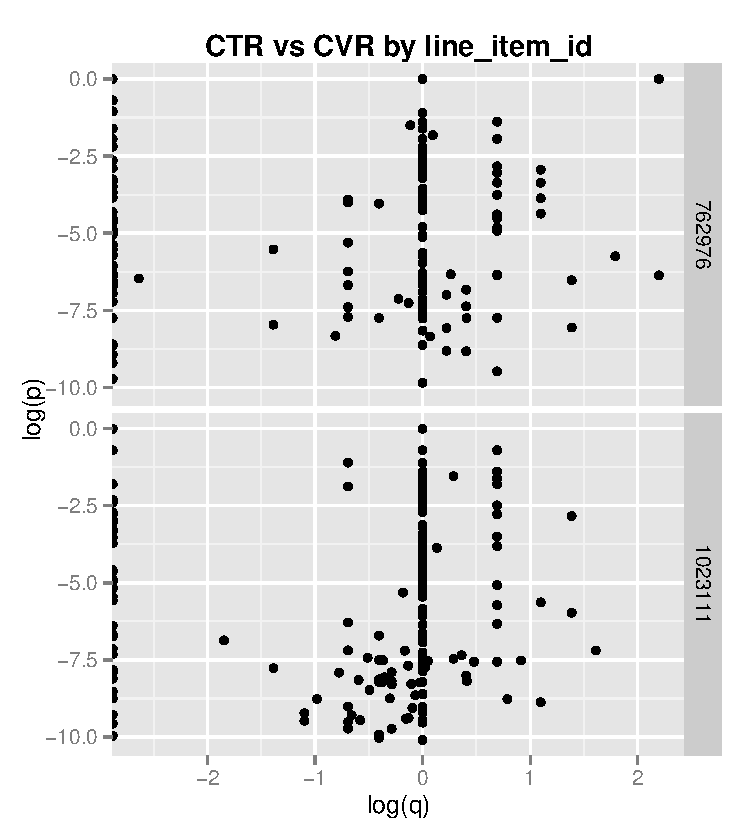
\includegraphics{CTRvsCVR}
    \caption{CTR against CVR by campaign}
    \label{fig:CTRvsCVR}
\end{figure}


Note the points on the far left of the plots have value q==0.  We see that CTRs take a broad range of values and CVR has less variation. 

\subsection{data cleaning}

When aggregated through the lifetime of the campaign we can get examples where $a>c$ due to the same visitor generating multiple "conversion events" by accidentally refreshing their page.

We produce a 'clean' version of the data set by removing all examples with $a_i > c_i$ or $c_i > n_i$. Though in our correlation analysis we choose not to use the original data set as we lose too many examples with acquisitions.

\subsection{CTR CVR dependency}

The relationship between CTR and CVR is not obvious, we look at various ways to focus on important relationships that may be obscured - weighted correlation, focusing on subgroups.


\chapter{Binomial Data Models}

We begin by exploring a variety of models for binomial data, motivated by our understanding of the RTB problem. In the next section we will explore how these models help optimise our campaign goals and inform decision policy.

Our goal with these models is to help generate acquisitions by exploring the model, so we will be asking questions such as:
\begin{itemize}
	\item How many data points would we need to fit the model.
	\item What does one arm tell us about another.
	\item Does the model help avoid chasing noise.
	\item Do clicks help make inference about acquisitions.
\end{itemize}

% If they are dependent, we consider 2 types of dependency - a cluster based dependency where the maximum likelihood value of q will jump between 2 values as p varies, and a correlation model where the ML value of q will vary smoothly as a function of p.

% Danaher et al ~\cite{danaher2005bacon}, Kupper ~\cite{kupper1978use} and Lee ~\cite{ting1996properties} provide smooth correlation models between p and q.

% An exact test for beta-binomial model is non-trivial, Garren et al ~\cite{garren2001bootstrap} has an excellent review of goodness-of-fit tests for beta-binomial model. Where as Mantel et al ~\cite{mantel1987goodness} addresses our issue of varying sample sizes ($n$).


\section{Model definitions} 


We start with simple binomial model (m1), then look to beta binomial (m3) to deal with over-dispersion. We then bring in intermediate clicks, hoping these can offer more information on the likelihood of future acquisitions. We discuss under what conditions clicks provide information on acquisitions in the appendix. We consider both cluster models as well as a correlation models to describe dependency between p and q.

\begin{description}
	\item[Model 1 - Single Binomial]
All arms are assumed to have the same reward function. We assume a uniform Beta prior so that the MAP estimate of a is equivalent to the MLE and is also an unbiased estimator. We gain as much information about lever 1 by looking at lever 2 as by looking at lever 1.

  \begin{align}
	a_i \sim Bin(q,c_i) \\
	c_i \sim Bin(p,n_i) \\
	\pi(q) \sim Beta(1,1) \\
	\pi(p) \sim Beta(1,1) 
  \end{align}

	\item[Model 2 - Independent Binomials]
Here we take $\alpha, \beta$ values to be known fixed values (possibly based on previous campaigns), thereby making all $q_i$ and $p_i$ values independent of each other. There is no information to be gained about lever 1 by looking at lever 2.

  \begin{align}
	a_i \sim Bin(q_i,c_i) \\
	c_i \sim Bin(p_i,n_i) \\
	\pi(q_i) = Beta(\alpha_q,\beta_q) \\
	\pi(p_i) = Beta(\alpha_p,\beta_p) \\
  \end{align}

Within this model, we also have the option to use regressors such as campaign type to offer different $\alpha, \beta$ values to different classes of arm without changing the posterior update procedure.

	\item[Model 3 - Beta-binomial]


% Useful if data not completely independent but is over dispersed for a binomial model. Here we assume a hierarchical model where the conversion rate for each arm is sampled from a Beta distribution with common $\alpha$, $\beta$ parameters across all arms. 

We now take M2 and assume that $\alpha, \beta$ values are random variables, rather than being fixed. In a sense, this model lies somewhere between model 1 and model 2, in that data about lever 1 gives us some information about lever 2 via inference of shared $\alpha$, $\beta$ parameters. 

  \begin{align}
	a_i \sim Bin(q_i,c_i) \\
	c_i \sim Bin(p_i,n_i) \\
	q_i \sim Beta(\alpha_q,\beta_q) \\
	p_i \sim Beta(\alpha_p,\beta_p) \\
	\pi(\alpha_q) = \pi(\beta_q) = \pi(\alpha_p) = \pi(\beta_p) = 1
  \end{align}

The benefit over model 2 is that we can update shared $\alpha, \beta$ values online, and therefore require less sample data to fit the correct AQR should our M2 priors be incorrect. The cost is that the posterior distribution of $p_i$ and $q_i$ no longer has an analytic form and we must use Monte Carlo methods to sample.

As with M2, we have the option to use regressors to offer different $\alpha, \beta$ variables to different classes of arm.

% When p and q are independent of each other, $a_i$ has distribution $Bin(p_iq_i,n)$ and $p_iq_i$ has distribution $Beta(a_i,n_i - a_i)$ (see 'Do Clicks Matter' for proof).  The intuition here is that clicks are not informative - as much as they increase our belief in click through rate, they decrease our belief in the acquisition rate.

	\item[Model 5 - 2 cluster Binomial]

Model 3 assumed that CTR and CVR are independent. Experience suggests that levers tend to perform well on both CTR and CVR or poorly on both. In other words, there tend to be 'clusters' of good and bad levers. Model 5 attempts to capture this with a binomial mixture model. We use priors to bias one cluster towards being the poor performer, this helps avoid 'index switching' complications with model fitting. 
 
 \begin{align}
	k \sim Bern(h) 
\end{align}
	\[ 
	a_i = 
  	\begin{cases}
		Bin(q_0,c_i) & \quad \text{if k is 0}\\
		Bin(q_1,c_i) & \quad \text{if k is 1}
	\end{cases}
	\]
	\[
	c_i = 
  	\begin{cases}
		Bin(p_0,n_i) & \quad \text{if k is 0}\\
		Bin(p_1,n_i) & \quad \text{if k is 1}\\
	\end{cases}
	\]

 \begin{align}
	\pi(h) = Unif(0,1) \\
	\pi(p_0) = \pi(q_0) = Beta(1,10) \\
	\pi(p_1) = \pi(q_1) = Beta(10,1) \\
\end{align}

%
%	\item[Model 6 - 2 cluster Beta-binomial]
%
% \begin{align}
%	a_i \sim Bin(q_i,c_i) \\
%	c_i \sim Bin(p_i,n_i) \\
%	k \sim Bern(h) 
%\end{align}
%	\[ 
%	q_i \sim 
%  	\begin{cases}
%		Beta(\alpha_{q0},\beta_{q0}) & \quad \text{if k is 0}\\
%		Beta(\alpha_{q1},\beta_{q1}) & \quad \text{if k is 1}
%	\end{cases}
%	\]
%	\[
%	p_i \sim 
%  	\begin{cases}
%		Beta(\alpha_{p0},\beta_{p0}) & \quad \text{if k is 0}\\
%		Beta(\alpha_{p1},\beta_{p1}) & \quad \text{if k is 1}\\
%	\end{cases}
%	\]
%
% \begin{align}
%	\pi(h) \sim Unif(0,1) \\
%	\pi(\alpha_{q0}) \sim Gamma(1,2) \\
%	\pi(\beta_{q0}) \sim Gamma(1,2) \\
%	\pi(\alpha_{p0}) \sim Gamma(1,2) \\
%	\pi(\beta_{p0}) \sim Gamma(1,2) \\
%	\pi(\alpha_{q1}) = \pi(\beta_{q1}) = \pi(\alpha_{p1}) = \pi(\beta_{p1}) = 1
%\end{align}
%
% TODO
% 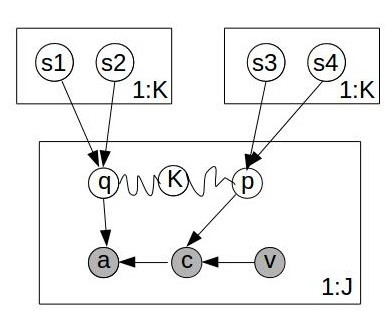
\includegraphics{GraphMod.jpg}

	\item[Model 7 - Correlated Beta-binomial]

As an alternative to model 6, where rate prediction will change abruptly between clusters, we look for a model where q can vary smoothly as a function of p.

\end{description}


\section{Generated data plots}

To generate the data for each model, we first sampled $n$ from the Advance media data set. This minimises issues around modelling the distribution of n. $c$ and $a$ were then generated randomly based on the model parameters.


\begin{figure}[p]
    	\centering
	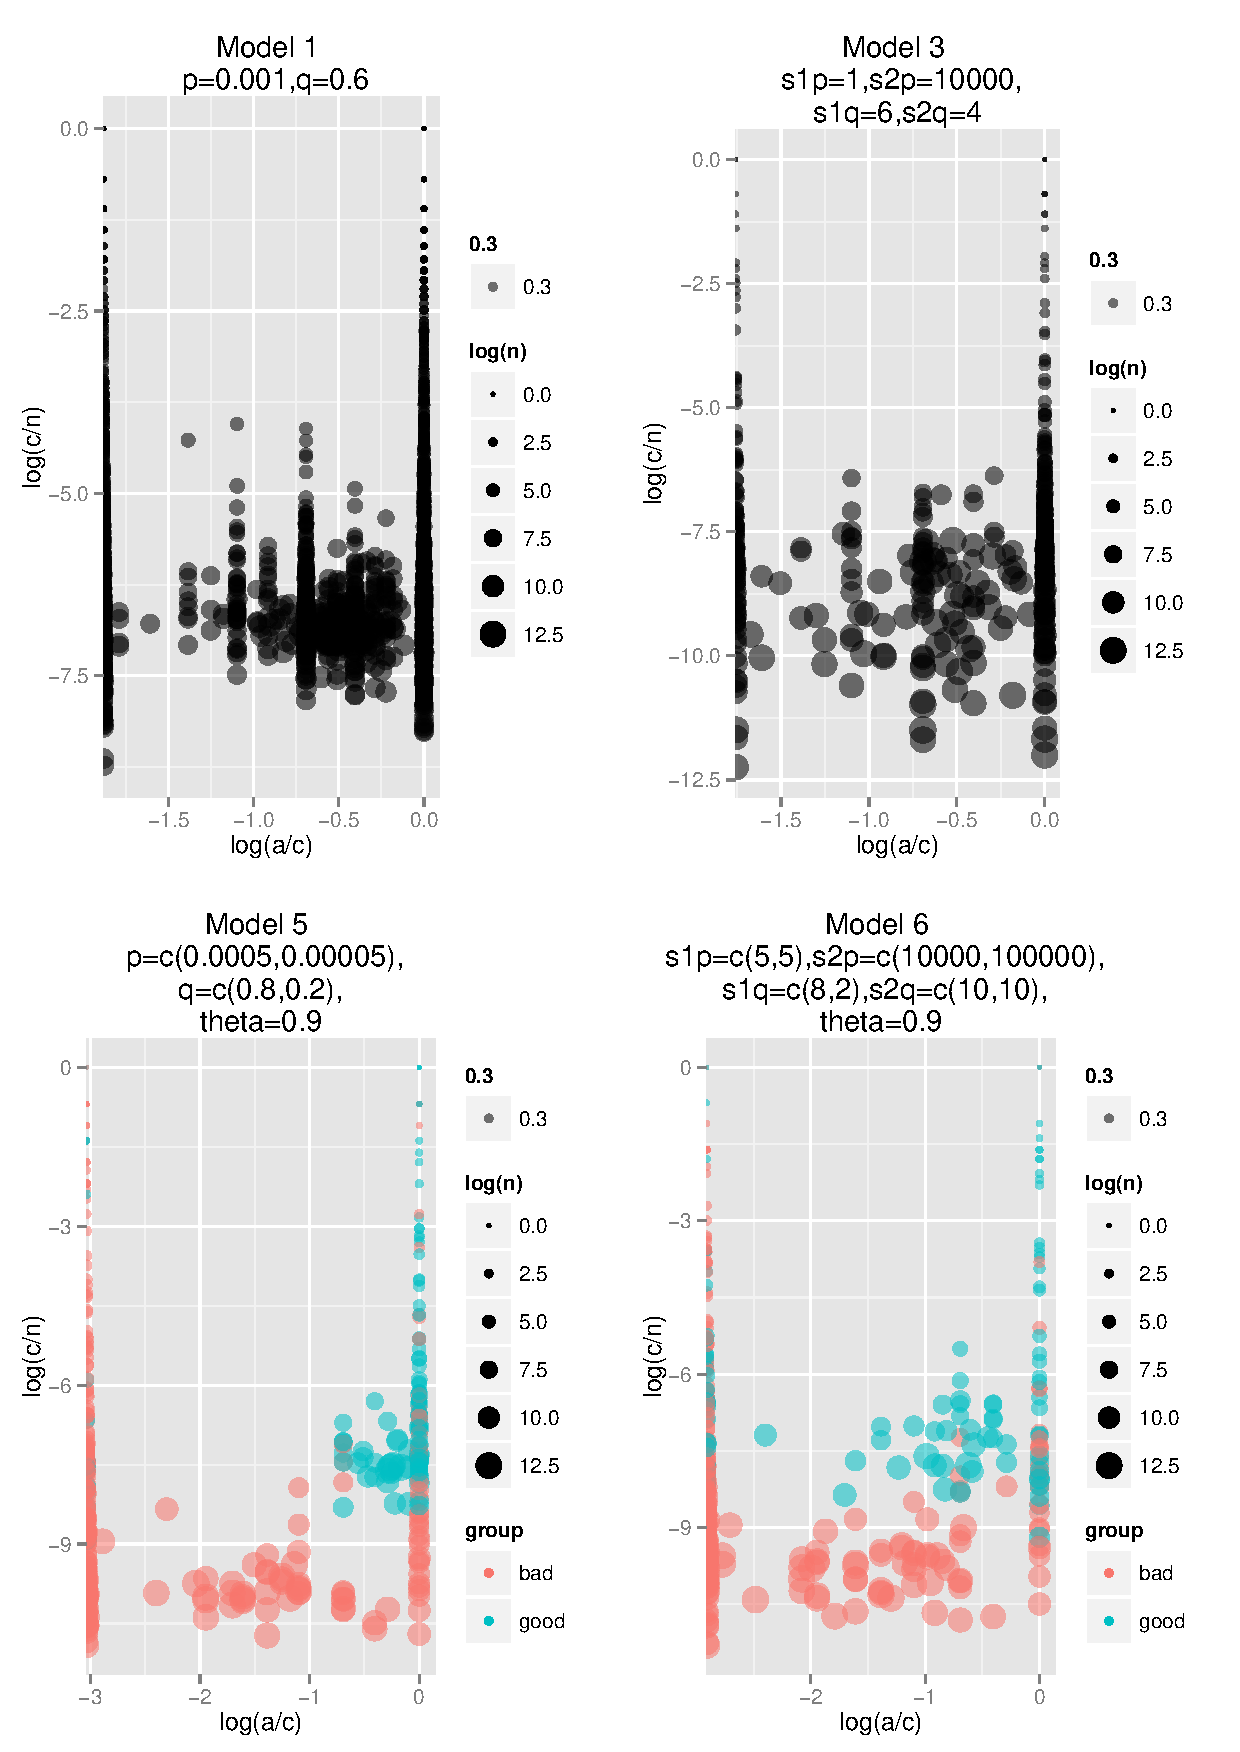
\includegraphics[scale=0.7]{SynthData}
    	\caption{Model generated data}
    	% \label{fig:GIvsUCB1}
\end{figure}




\section{Test methodology} 

\subsection{ Correlation measures}

A dependency between CTR and CVR would be a big benefit in predicting AQR since clicks are more common than acquisitions. We define a few measures of correlation below. We apply these to the model generated data sets to see if they help distinguish the relationships present in m5 and m6 from the independent models m1 and m3. We also apply the measures to the Advance data set for comparison with the 4 models.

\begin{description}
	\item[Cor] Pearson correlation coefficient between CVR ($a/c$) and CTR ($c/n$).
	\item[IWC] Impression weighted correlation - a Pearson correlation coefficient weighted by the number of impressions ($n$). This measure is intended to reduce some of the noise coming from the many sites with few impressions. Possible values range from 0 to 1.
	\item[logIWCc] Impression weighted correlation between log(CVR) and log(CTR).Possible values range from 0 to 1.
	\item[RankCor] Spearman's rank correlation between CVR and CTR.
	\item[glmcoef] We fit a binomial regression model as another way to measure Pearson correlation with reduced weight from small sample data points. glmcoef is the coefficient of CTR in this model:
	$(a,c) \sim log(CTR)$ 
	\item[glmsignif] The significance level associated with glmcoef.
\end{description}


\subsection{Goodness of fit tests}

We take the approach of starting with a simple model and run further tests to decide whether there is evidence to expand the model. 

Where possible we prefer tests with strong theoretical backing, e.g. LR. As model complexity rises it becomes harder to rely on these. We use information criteria and posterior validation.

\begin{description}
	\item[test 1] 

We assume the Normal approximation to the binomial and perform a chi squared test on the residuals, $r_i$ defined below:

\begin{align}
	\hat{q} = \frac{ \sum_{i} a_i }{ \sum_{i} n_i } \\
	r_i = \frac{ a_i - n_i \hat{q} }{ a_i \hat{q} (1 - \hat{q}) }
\end{align}

Since the Normal approximation only holds for large c, so we group all examples with the values of c less than 10.


%
%A frequentist style goodness of fit test designed to assess whether data can be well explained with simple binomial model 1. We use the binomial approximation to the Normal and perform pearson chisq on the residuals. This only holds for large n, so we group the small n values to test whether (together) they share the same mean.
%
%Benefits are that we can have a composite alternative hypothesis, downside is the approximation used. Could be improved by Yates' corerction. 
%% TODO - approximation fails for p as rate is very small.


	\item[test 2] 

We construct a likelihood ratio test statistic $D$ comparing null hypothesis Model 1, with the alternate hypothesis Model 3. We use the VGAM package to find ML estimates for m3 and validate this with the same model constructed with RStan. 

\begin{align}
	D = -2 \max_{q} \sum_i \log( \operatorname{Bin}(a_i;c_i,q) ) +
	2 \max_{\alpha,\beta} \sum_i \log( \operatorname{BetaBin}(a_i;c_i,\alpha,\beta) ) 
\end{align}

Our argument for using this test here is that:
\begin{align}
	 \operatorname{BetaBin}(a;c,pn,(1-p)n) \overset{d}{\to} \operatorname{Bin}(a;c,p) \quad \operatorname{as} \quad n \to \infty
\end{align}

%Assuming we reject model 1, we try LR test to see if data is better modelled using beta-binomial. Testing null hypothesis against all others is difficult. LR test has the benefit of being 'most powerful' for comparing 2 point hypotheses, so is a good choice assuming we are happy using ML point hypotheses. If we were willing to specify priors on parameters, we could turn this in to a Bayes factor test.
%
% TODO - compare ratio value to alpha, or do chisq on deviances?


	\item[test 3] We create 2 hypothetical groups split based on the median realised acquisition rate. We create a binary variable $X$ for membership of this group. We then use binomial regression to fit 1 and 2 cluster models:

\begin{align}
	M_0 := (a,c) \sim 1 \\
	M_a := (a,c) \sim X + 1
\end{align}

We then construct a likelihood ratio test comparing $M_0$ with $M_a$. 

We choose this test because it is easy to set up and may indicate clustering. A more accurate test would use EM to assign data points to clusters.
%
%LR test Model 1 vs Model 5 - 1 cluster binomial vs 2 cluster binomial. In fitting the 2 cluster model, we visually split the data and fit 2 separate binomials, so the test is only approximate. 
%
%
%	\item[test 4] Assuming we reject the null in test 2, due to over dispersion, we check if can extend this to 2 cluster model with another LR test. In fitting the 2 cluster model, we visually split the data and fit 2 separate beta-binomials, so the test is only approximate. 
%
%Obviously we could keep testing for additional clusters. A more general approach could be to define prior penalizing large number of clusters and use VB or Gibbs to find posterior.
%
\end{description}

\section{Results}
\subsection{Correlation measures}

% Created by running Results.R

% latex table generated in R 3.0.2 by xtable 1.7-3 package
% Wed Sep 17 21:40:26 2014
\begin{table}[ht]
\centering
\begin{tabular}{rlrrrrrrrr}
  \hline
 & Dataset & Cor & IWC & logIWCc & RankCor & items & imps & glmcoef & glmsignif \\ 
  \hline
  1 & Advance & -0.07 & 0.03 & 0.10 & 0.20 & 191 & 23228621 & -0.04 & 5.2E-02 \\ 
  2 & m1 & -0.00 & -0.01 & -0.03 & 0.02 & 1573 & 13231538 & 0.12 & 6.3E-04 \\ 
  3 & m3 & 0.05 & -0.00 & -0.05 & 0.05 & 345 & 13791746 & -0.02 & 6.7E-01 \\ 
  4 & m5 & -0.12 & 0.04 & 0.37 & 0.17 & 337 & 12789708 & 0.66 & 1.1E-43 \\ 
  5 & m6 & -0.03 & 0.04 & 0.25 & 0.02 & 324 & 13738487 & 0.29 & 3.9E-16 \\ 
   \hline
\end{tabular}
\end{table}

\subsection{Goodness of fit}

Here we present p values for the 3 tests defined earlier.
% latex table generated in R 3.0.2 by xtable 1.7-3 package
%% Thu Sep 18 14:42:56 2014
\begin{table}[ht]
\centering
\begin{tabular}{rlrrrrr}
  \hline
 & Dataset & test1 & test2 & test3\_30 & test3\_45 & test3\_60 \\ 
  \hline
  1 & Advance & 0.00 & 0.00 & 1.00 & 1.00 & 1.00 \\ 
  2 & m1 & 1.00 & 1.00 & 0.00 & 1.00 & 1.00 \\ 
  3 & m3 & 0.00 & 0.00 & 0.00 & 1.00 & 1.00 \\ 
  4 & m5 & 0.00 & 0.00 & 0.00 & 0.00 & 1.00 \\ 
  5 & m6 & 0.00 & 0.00 & 0.00 & 0.00 & 1.00 \\ 
   \hline
\end{tabular}
\end{table}

%  \hline
%  1 & Advance & 0.00 & 0.00 & 1.00 & Error \\ 
%  2 & m1 & 1.00 & 1.00 & 1.00 & Error \\ 
%  3 & m3 & 0.00 & 0.00 & 1.00 & Error \\ 
%  4 & m5 & 0.00 & 0.00 & 1.00 & Error \\ 
%  5 & m6 & 0.00 & 0.00 & 0.00 & 0 \\ 
%   \hline

\section{Summary}

We see that the logIWCc is the best performing correlation measure, with a strong response to the two dependency models, and weak response to m1 and m3. Rank correlation seems to identify the dependency in m5, but miss m6 where the clusters are less sharply peaked (see data plots). Logistic regression clearly identifies the correlation present in m5 and m6, though also suggests m1 has a significant dependency, which it should not. This would need further investigation were we to use this measure.

What this means for the Advance data is inconclusive, though rank correlation suggests there is a dependency, logIWCc is weaker and binomial regression even suggests a slight negative correlation.

Test 1 suggests we should reject the binomial model for all but m1, as we would expect.
Test 2 says we should prefer the beta binomial model for all but m1, as we would expect. 
Test 3 turns out to be a poor tool. Although with a value of .45 we get sensible results, it is very sensitive to our choice of boundary to split the clusters.

% TODO Test 4 can't fit the data.

%\begin{itemize}
%	\item Need to use log values of p.
%	\item Clustering based on $a_i$ creates false correlations.
%	\item Clustering based on c does not create false correlations.
%	\item Using c greater than 0, correlations do not show up. But become stronger for c gt 1, c gt 2. This is because it reduces the noise of all the small-n zero and one values.
%	\item Filter based on realized CTR is no use as it does not help with (3). Needs a correlation measure which properly accounts for likelihood weight of response - closest thing is glm.
%	\item Binomial GLM does the best job of (4), though does not consider error in dependent variable.
%\end{itemize}
%

\chapter{ Sequential Decision Policies }

\section{ Markov Decision Processes }

A Markov decision process is a formalism for describing sequential decision problems in discrete time. An MDP consists of a 4-tuple of states $\mathcal{S}$, actions $\mathcal{A}$, state transition probabilities under each action $P_a(s,s')$, and reward distributions for the each transition $\mathcal{R}_a(s,s')$. The goal is to seek policy $\pi$ which maximises the rewards over the lifetime of the process. For each time $t$:

\begin{align}
a_t &\in \mathcal{A} \\
s_t &\in \mathcal{S} \\
r_t &\sim \mathcal{R}_{a_t}(s_t,s_{t+1})
\end{align}

The figure below visually represents a 3 state MDP, with 2 available actions.

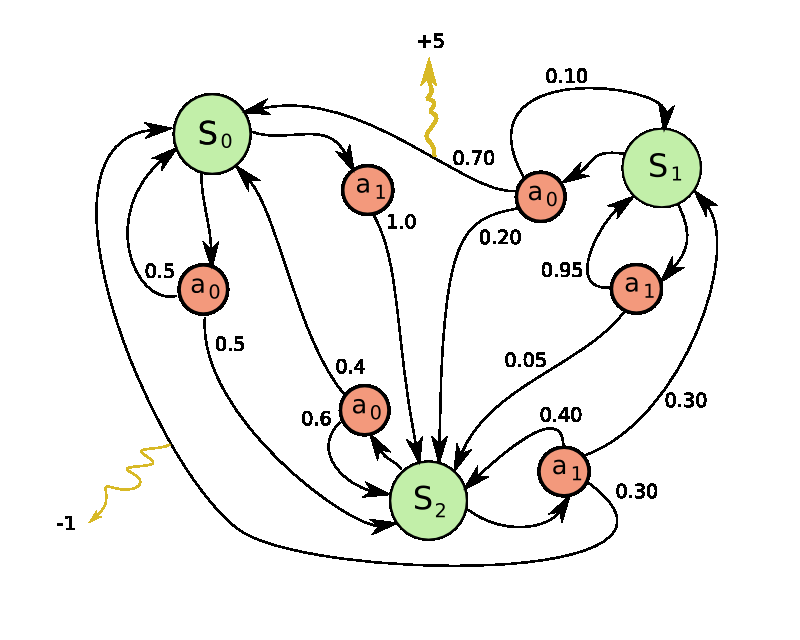
\includegraphics[scale=0.5]{MDP_example.png}

Figure attribution: "Markov Decision Process example" by MistWiz - Own work. Licensed under Public domain via Wikimedia Commons - 

http://commons.wikimedia.org/wiki/File:Markov\_Decision\_Process\_example.png\#

mediaviewer/File:Markov\_Decision\_Process\_example.png

\subsection{ Dynamic programming and optimal control }

For a finite number of time steps, MDPs have optimal policies defined by the Bellman equation. The dynamic programming equation assigns a value to each action equal to the expected immediate reward plus the expected future rewards $V$ of the state transitioned to, under an optimal policy.

The optimal policy is then to greedily choose action with highest value.

\begin{align}
	V(s_0) &= \max_{a \in \mathcal{A}} E_{s'}[\mathcal{R}_a(s_0,s')] \\
	V(s_t) &= \max_{a \in \mathcal{A}} E_{s'}[\mathcal{R}_a(s_t,s') + V(s')]
\end{align}

\subsection{ Q-learning }

When the rewards are unknown, this becomes the reinforcement learning problem. Q-learning ~\cite{watkins1992q} is a popular framework for iteratively estimating the state-action value function defined by the Bellman equation. Here $Q_t$ is our estimate of the value function, and $\alpha$ is a 'learning rate' parameter:

\begin{align}
Q_{t+1}(s_t,a_t) = Q_t(s_t,a_t) + \alpha\{r_{t+1} + \max_a Q_t(s_{t+1},a) -Q_t(s_t,a_t)\}
\end{align}

Q-learning is 'model free' in that it makes no explicit assumptions about the relationship between actions, states and rewards. It can also be used in conjunction with a linear function approximation ~\cite{tsitsiklis1997analysis}, or sophisticated neural-net ~\cite{mnih2013playing}. This can make large models more tractable.

The algorithm also requires an explicit policy for exploring sub-optimal actions, such as $\epsilon$-greedy (see section ~\nameref{sec:heuristics}).

\section{ Multi-armed bandits and regret}

A multi-armed bandit is a single state MDP with unknown rewards. It has K actions, or 'arms'. The name comes from the analogy with choosing how to bet on a choice of K slot machines, which are sometimes known as one-armed bandits.

\begin{align}
&\mathcal{A} = \{1,...,K\} \\
&a \in \mathcal{A} \\
&r_t \sim \mathcal{R}_{a_t} 
\end{align}

Typically bandits policies are assessed by how well they minimise \textit{regret}. The regret of policy $\pi$ is defined as the expected difference from the \textit{oracle} policy of always choosing arm with maximum expected reward:

\begin{align}
&\mu_a = E[r|a] \\
&\mu^{*} = \max_{a \in \mathcal{A}} \mu_a \\
\operatorname{regret}(\pi) &= \sum_{t=1}^T (\mu^{*} - \mu_{\pi(t)})
\end{align}

\section{PAC learning}

PAC learning approaches look to limit the number of sub-optimal decisions. But this pure exploration approach does not naturally map to our goal of maximising value from our campaign budget.

\section{ Bayes Adaptive policy }

For given priors, it is possible to define a 'Bayes-optimal' policy. A MAB problem is a one state MDP with unknown rewards. We can turn this in to a many state MDP with known rewards by representing each possible posterior value as a new state. Each transition probability is given it's expected value based on the current posterior. This idea is present in early discussions of sequential binomial decision problems ~\cite{chernoff1965bayes} but has more recently been labelled Bayes adaptive reinforcement learning in machine learning literature ~\cite{duff2002optimal}. Now that we know the action rewards and transition probabilities, the optimal decision policy is provided by the Bellman equation. Appendix provides an example of how this is calculated.

The graphs below provide a demonstration of this policy. In each graph, we see which arm is optimal as a function of rounds remaining. Note the high expectation arm is preferred for short campaigns and changes toward the high variance arms as the time horizon increases. The 6 panes show one possible scenario play out as arms are chosen and posteriors are updated.


\begin{figure}[p]
    \centering
    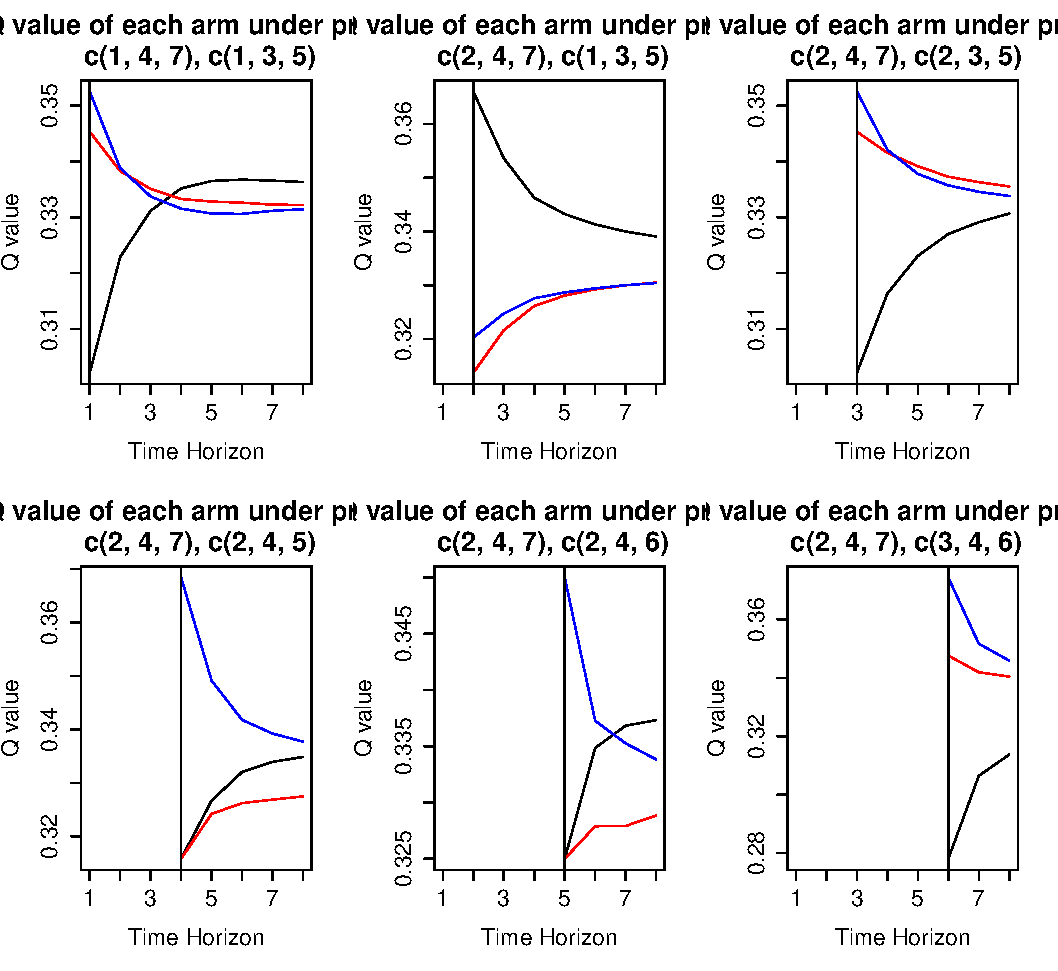
\includegraphics[scale=0.7]{BARLillustration.pdf}
    \caption{Bayes Adaptive reinforcement learning solutions}
    % \label{fig:GIvsUCB1}
\end{figure}


This solution has a number of particularly attractive characteristics over probability matching strategies such as Thompson sampling and UCB:
\begin{itemize}
	\item We see that for small numbers of rounds, the algorithm purely exploits the high expectation arms, since there are too few rounds for the high variance arms to produce enough positive results to change our decisions. This is very relevant for our domain where we may have millions of arms (sites x placements x creatives x userType) but only a few 100,000 rounds and expectation of only a few 100 acquisitions. This addresses the issues we saw in previous section where the click only model would benefit from early exploitation of non-optimal arms. Thompson sampling and UCB would typically over explore in these situations too.
	\item We can still integrate our prior information.
	\item If arms have some common dependency, such as using the same creative it understands there is greater exploration value.
	\item Policy responds to changes how we value events, underlying model, time horizons etc.
	\item The approach is orthogonal to the underlying model, so that we can develop the underlying model without needing to update the decision algorithm.
\end{itemize}

The limiting factor for this approach is that the algorithm has exponential order cost and so can be computed exactly only for small games. Various sampling based approximations exist ~\cite{guez2012efficient}.

\section{ Heuristics } \label{sec:heuristics}

There are a variety of heuristic approaches, these tend to be simple to calculate and often provide tunable parameters though have no theoretic guarantees. See Scott ~\cite{scott2010modern} for a more extensive overview.

\begin{itemize}
	\item $\epsilon$-greedy - choose arm with highest expectation $\epsilon$ times, then choose a sub-optimal arm for exploration. The $\epsilon$ value can decrease over the life of the game.
	\item POKER ~\cite{vermorel2005multi} - attempts to assign an exploration value to each arm. It makes a number of assumptions to estimate the probability the arm offers an improvement and the size of that improvement. The exploration value is then the probability weighted improvement multiplied by the number of rounds remaining to exploit it. Although it aims to capture the qualities we would expect in a good decision policy, in our view it does this artificially through the assumptions it makes. By comparison, these qualities arise quite naturally from the dynamic programming solution.
\end{itemize}

\section{ Thompson Sampling }

Thompson sampling is a non deterministic strategy. The policy chooses arm $j$ with frequency $w_j$, which is the posterior probability that it is the optimal arm.

\begin{align}
w_j = P(\mu_j > \max(\mu_1, ..., \mu_k))
\end{align}

Agrawal and Goyal ~\cite{DBLP:journals/corr/abs-1111-1797} prove asymptotic optimality for the binomial case, as well as demonstrate finite horizon performance improvement over KL-UCB and UCB using simulation studies.

\section{ Gittins Index }

Gittins ~\cite{gittins1979bandit} was able to show that the MAB problem with geometrically discounted regret could be treated as an index problem, meaning that the optimal decision rule is to select arm with highest index. That index could be calculated using only information about the arm. The intuition here is that since playing one arm does not affect the rewards of other arms, a value can be computed using only information about that arm. The value is the expected rate of reward under an optimal stopping rule.

\begin{align}
v(s) = \sup_{\tau > 0} E\left[ \sum_{t=0}^{\tau-1} b^t \mathcal{R}(s_t) | s_0 = s  \middle/  E\left[ \sum_{t=0}^{\tau-1} b^t | s_0 = s \right]  \right]
\end{align}

Although the Gittins index is not optimal in the finite horizon case (the value of alternate arms changes as a result of the loss of 1 round), it is a very close approximation. Our testing (not presented) confirms that GI and BA strategies achieve near equal regret.

As the calculation involves only 1 arm, the computation has significantly lower order, with the potential to share results between arms. Comparing the the Bayes Adaptive solution $O((\#\mathcal{A} \#\mathcal{P})^T)$, we instead have:

\begin{itemize}
	\item $O(\#\mathcal{A} {\#\mathcal{P}}^T)$ - Exact method.
	\item $O(\#\mathcal{A} T^{\#\mathcal{P}})$ - Calibration method.
\end{itemize}

\subsection{ Exact method }

Gittins 1979 ~\cite{gittins1979bandit} describes an exact method for calculating the index for a finite horizon. 

The calculation of this index typically involves choosing a number of rounds to look ahead. In infinite horizon game, the less the discount factor, the more rounds are required to get a close approximation. Then calculate the value at round N and use backwards induction to calculate the value for round 0.

\subsection{ Calibration method }

There are several methods looking for more computationally efficient calculation, the most popular being the calibration method where a grid of candidate GI values is used to obviate the need to recurse. See Nino-Mora ~\cite{nino2011computing} for an overview. The cost for these methods is still exponential in the order rounds and so will not scale to say a million rounds without some approximations used.

We demonstrate in the appendix that it is simple to adapt the GI for binomial bandits to the models involving independent clicks and acquisitions as it only requires taking expectations. Note that since this is a finite horizon game, there is no loss of accuracy associated with calculating a finite number of rounds.

\subsection{ Approximations }

Noting that GI is a function of only 5 variables, we consider approximations. Brezzi and Lai ~\cite{brezzi2002optimal} provide a closed form (i.e. constant order) solution to the infinite horizon problem using a Normal approximation by relating the discrete time problem to a continuous time Wiener process.  The same paper references Lai ~\cite{lai1987adaptive} for asymptotically optimal solutions for the finite horizon, undiscounted problem for single parameter exponential family distributions. Burnetas and Katehakis ~\cite{burnetas1996optimal} extend this to multi-parameter univariate distributions.

The multi-parameter solution would fit our both model well and provide opportunity to extend the funnel to include additional intermediate steps. Unfortunately, we note, our UCB and Thompson sampling testing finds these asymptotically optimal approaches do not work well with the arms, rounds and rates we work with.

\section{ Lai and Robbins lower bound }

Motivated by Gittins proof of the existence of optimal index policies, Lai and Robbins ~\cite{lai1985asymptotically} proved that a class of decision algorithms meeting certain conditions were asymptotically optimal learners. This insight is the basis for the deterministic probability matching, UCB algorithms. 

\begin{align}
\operatorname{regret}(\pi)  \leq  \frac{\ln(n)}{D_{KL}(\mu_j||\mu^{*})} \quad as \quad n \to \infty
\end{align}

We note that the optimal asymptotic regret leaves scope for a large constant regret term, as we found in our experiments poor performance over limited horizons. We conjecture that due to the high number of arms, and low success rate, in practise we do not get to the region where asymptotic behaviour dominates.

\section{ UCB1 }

There is a large family of index algorithms based on assigning an 'upper confidence bound' value to each arm. In these, we allow the estimated payoff $\hat{\theta}$ of the arm to increase up to a constraint based a maximum KL divergence of the parameter. The $\lambda$ value controlling the constraint will typically vary based on the number of times the arm has been played and the current round.

\begin{align}
v_j = \inf\{ \mu : \mu \geq \hat{\mu_j}, D_{KL}(\mu||\hat{\mu_j}) \geq \lambda\} 
\end{align}

Where $n$ is the current round, $n_j$ is the number of times arm $j$ has been played, UCB1 algorithm assigns the arm an index according to rule:

\begin{align}
v_j = \hat{\mu_j} + \sqrt{ \frac{2 \ln{n}}{n_j}  }
\end{align}

Agrawal and Goyal ~\cite{DBLP:journals/corr/abs-1111-1797}, in their analysis of Thompson sampling demonstrated superior performance from Thompson sampling compared to a variety of modern UCB algorithms for binomial problems.

\chapter{ Results }

\section{Test harness}

A simulation test harness was set up to simulate MAB trials. Custom policies were run in the harness and assessed by calculation of realised regret.

\begin{enumerate}
	\item Experimenter defines a bivariate Beta prior distribution parameterised by alpha and beta values for p and q.
	\item This prior is then used as a generative model to sample a set of 'true' p and q values for each arm.
	\item Each strategy is provided with the prior information and must infer the true values of p and q. The test harness calls on the strategy to return an arm number. The test harness then draws a single sample from a distribution using the true p and q values for this arm. The result is a tuple $(acquisition,click)$. The strategy is given this result so that it may update it's knowledge. The mean regret for the strategy is also updated.
	\item Step 3 is repeated for a set number of rounds i.e. the time horizon.
	\item Steps 2, 3 and 4 are looped 100 times so that we can calculate mean regret. Standard error for the mean values is estimated using a bootstrap method.
\end{enumerate}





\section{Thompson Sampling}

\begin{description}
	\item[ts\_clicks] Each arm is initialised with a beta prior using the alpha and beta values for p. Arms are chosen using Thompson sampling based on the probability of each arm having maximum p. The algorithm seeks to optimise clicks only, though regret is still calculated in same way.
	\item[ts\_both] Each arm is initialised with beta prior for both p and q. Arms are chosen using Thompson sampling based on the probability of each arm having maximum r value (i.e. pq). Since the distribution of pq does not in general have an analytic form, we use sampling. The priors on p and q are updated in the usual way.
	\item[ts\_acqs] The strategy only looks at acquisitions per view, ignoring clicks. Since the Beta priors on p and q do not directly translate in to a Beta prior on r, we estimate the parameters of a Beta prior for r using the mean and variance of p and q. This new Beta prior is updated in the usual way with acquisitions and views.
\end{description}

\subsection{Validation}

We run a set of validation checks to make sure we are not favouring one strategy in some extrinsic way - such as a more informative prior or more accurate posterior sampling.

\begin{enumerate}
	\item  We give p a point prior at value 1. With this, we expect to see the same performance from ts acqs and ts both. ts clicks should select arms arbitrarily.
	\item  We give q a point prior at value 1. With this, we expect to see the same performance from all 3 strategies as they are all 'learning' click rate.
	\item  We give both p and q flat priors. We expect to see the same performance from ts acqs and ts both as our analysis shows this is a special case, equivalent to modelling acquisitions only.
\end{enumerate}

\subsection{Plots}

\begin{figure}[p]
    \centering
    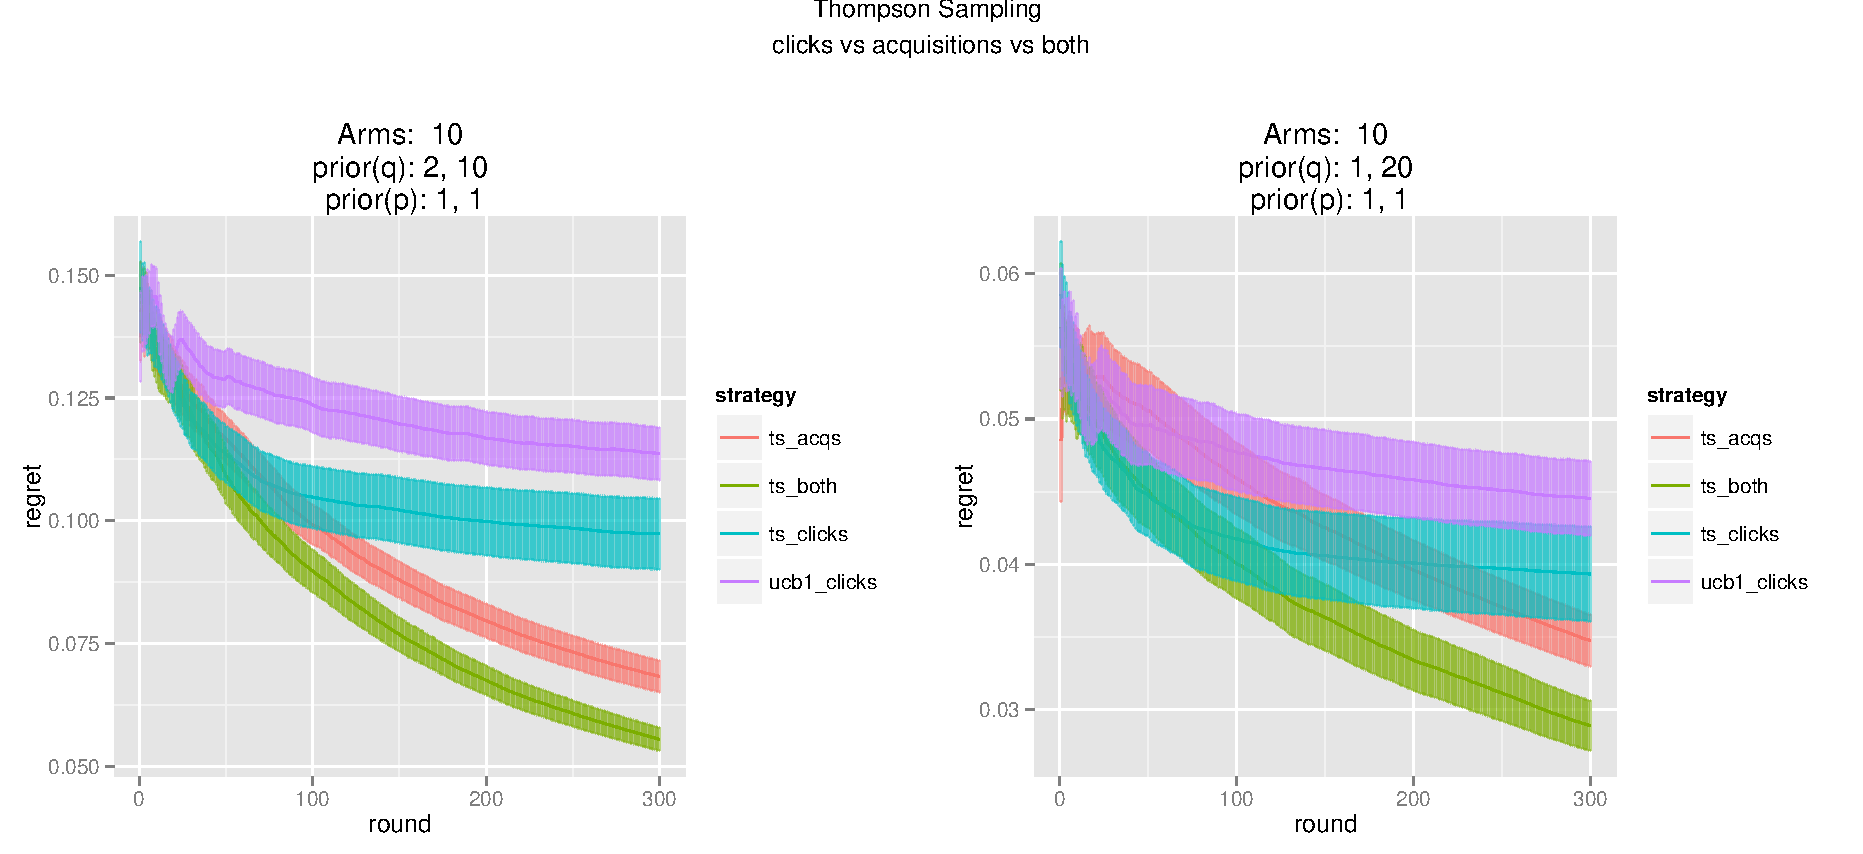
\includegraphics[scale=0.5]{P4to5UCB}
    \caption{Comparative regret of Thompson sampling versus UCB1}
    % \label{fig:GIvsUCB1}
\end{figure}

\begin{figure}[p]
    \centering
    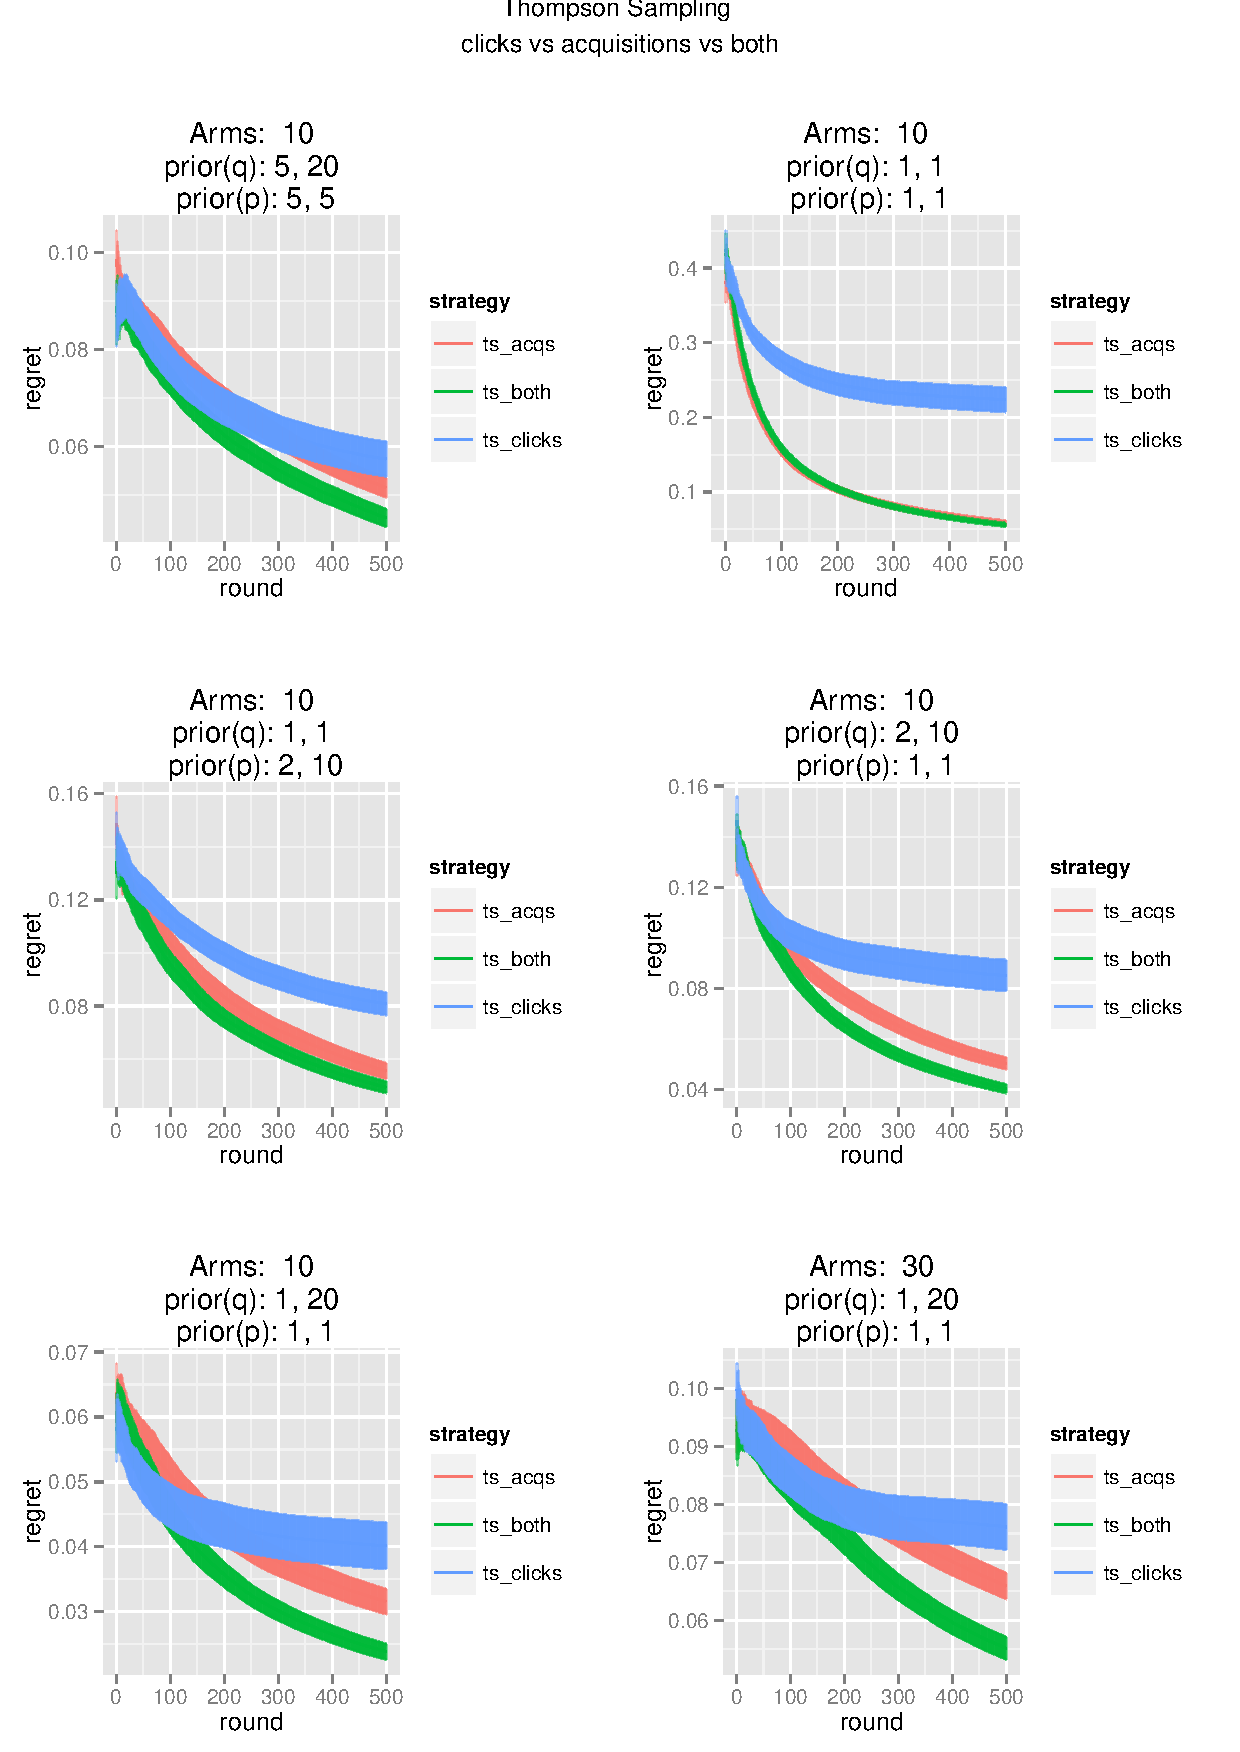
\includegraphics[scale=0.7]{P1to6.pdf}
    \caption{ Thompson Sampling performance varying priors }
    % \label{fig:GIvsUCB1}
\end{figure}




\subsection{Discussion}

\begin{description}
	\item[ts\_clicks] typically reduces regret very quickly particularly with few arms and high variance on p. But over longer periods loses out to ts acqs and ts both since the best arm does not always have the highest rate of clicks. If there is a high variance on q, it can go very wrong.
	\item[ts acqs] performs well for long trials or where q can take on high values. But typically learns slowly, particularly when q has small values.
	\item[ts\_both] robust to the pathological cases that see poor performance from ts clicks and ts acqs, and in certain cases produced significantly improved results on both. In all but one instance (discussed next), ts both is at least as good as either algorithm.

\end{description}

We also note that ts clicks initially beats ts both, though this advantage goes away once the number of arms is increased. We hypothesise this is a feature of Thompson sampling rather than the model - by ignoring some of the uncertainty in the true value of r, ts clicks gains an early exploitation advantage.

We also note that as the number of arms goes up, the regret increases. This could be because the 'best arm' becomes further from the average arm given more arms, but possibly a sign of over-exploration.


\section{ Bayes Adaptive }

The previous results demonstrated that a more sophisticated model offered stronger inference and could reduce MAB regret. But we also noted a couple of instances where performance was not as good as it might be. 

With this in mind, we now look at optimal decision rules incorporating the varying number of arms and campaign length.

\begin{description}
	\item[ba\_both] Each arm is initialised with beta prior for both p and q. Arm with maximum action value is always chosen, where multiple arms have same action value, one is selected at random.
	\item[ba\_acqs] The strategy only looks at acquisitions per view, ignoring clicks. Since the Beta priors on p and q do not directly translate in to a Beta prior on r, we estimate the parameters of a Beta prior for r using the a method of moment from the mean and variance of p and q. This new Beta prior is updated in the usual way with acquisitions and views. The arm selected is the one with maximum action value.
\end{description}




\subsection{Plots}

Using the same harness, we set up the experiment using a 'Bayes-optimal' exploration algorithm. Due to the exponential order cost of this algorithm, we must keep the games to a small number of rounds. 

\begin{figure}[p]
    \centering
    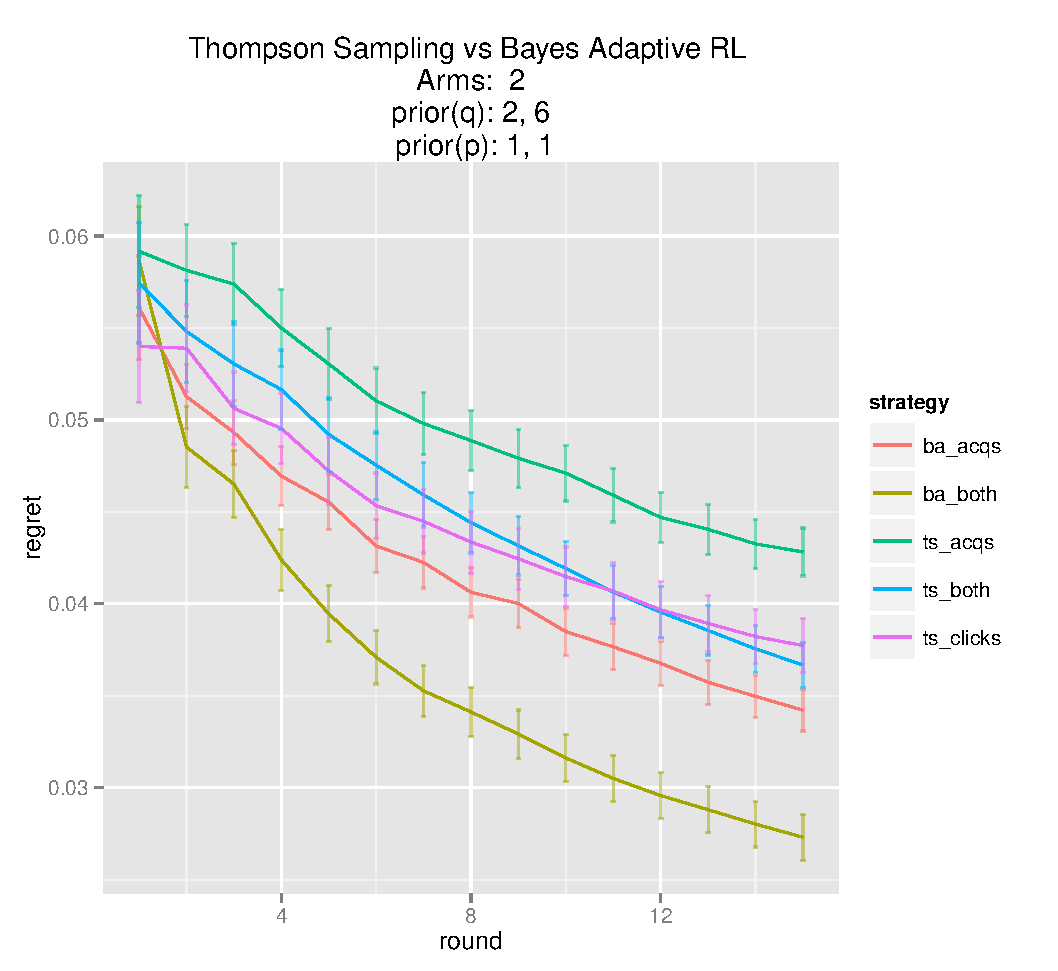
\includegraphics[scale=0.9]{TSvsBARL.pdf}
    \caption{ Thompson Sampling vs Bayes Adaptive RL }
    % \label{fig:GIvsUCB1}
\end{figure}



We see both Bayes Adaptive strategies improve on their Thompson Sampling equivalents. The strategy combining the improved model as well as the optimal decision policy offers very significant benefits.


\section{Gittins Index}

The Bayes-optimal solutions remain attractive. Although the Bellman equation gives us optimal solution, the computational time becomes prohibitive for large trials. We turn to GI solutions to provide nearly identical results with less computation.

\subsection{Plots}

\begin{figure}[p]
    \centering
    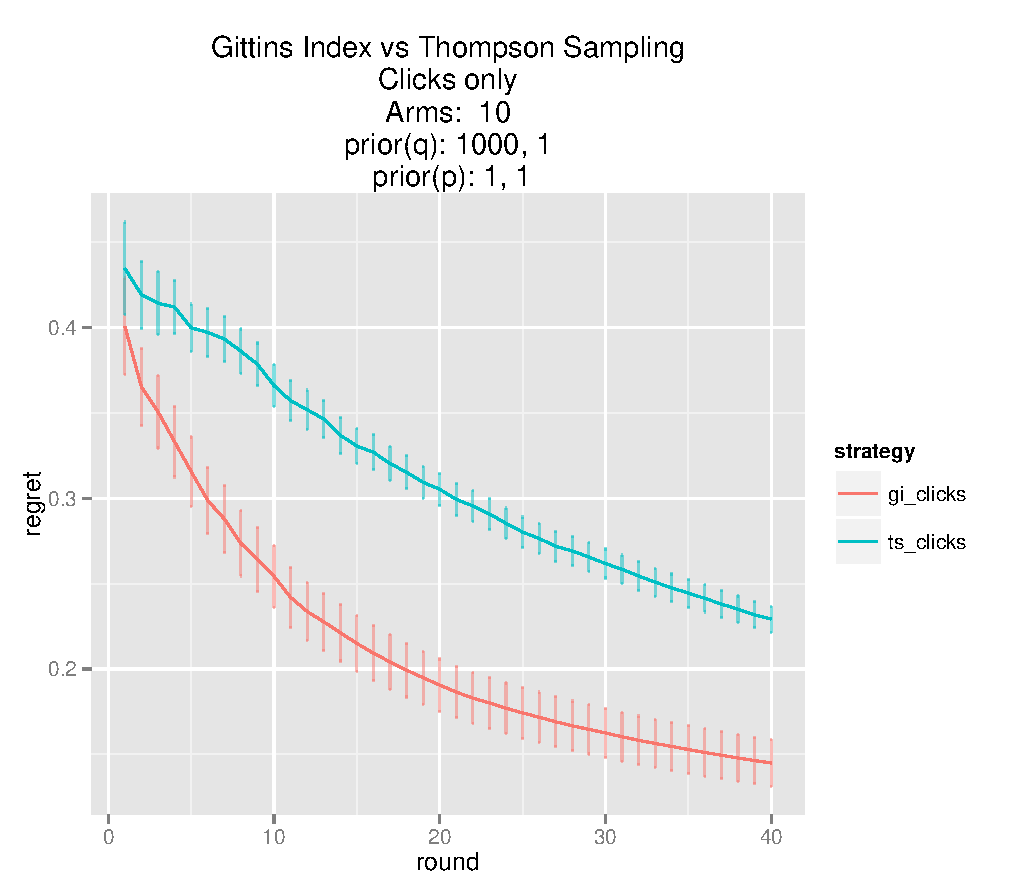
\includegraphics[scale=0.7]{GIvsTS.pdf}
    \caption{ Gittins Index vs Thompson Sampling - clicks only }
    % \label{fig:GIvsUCB1}
\end{figure}


\begin{figure}[p]
    \centering
    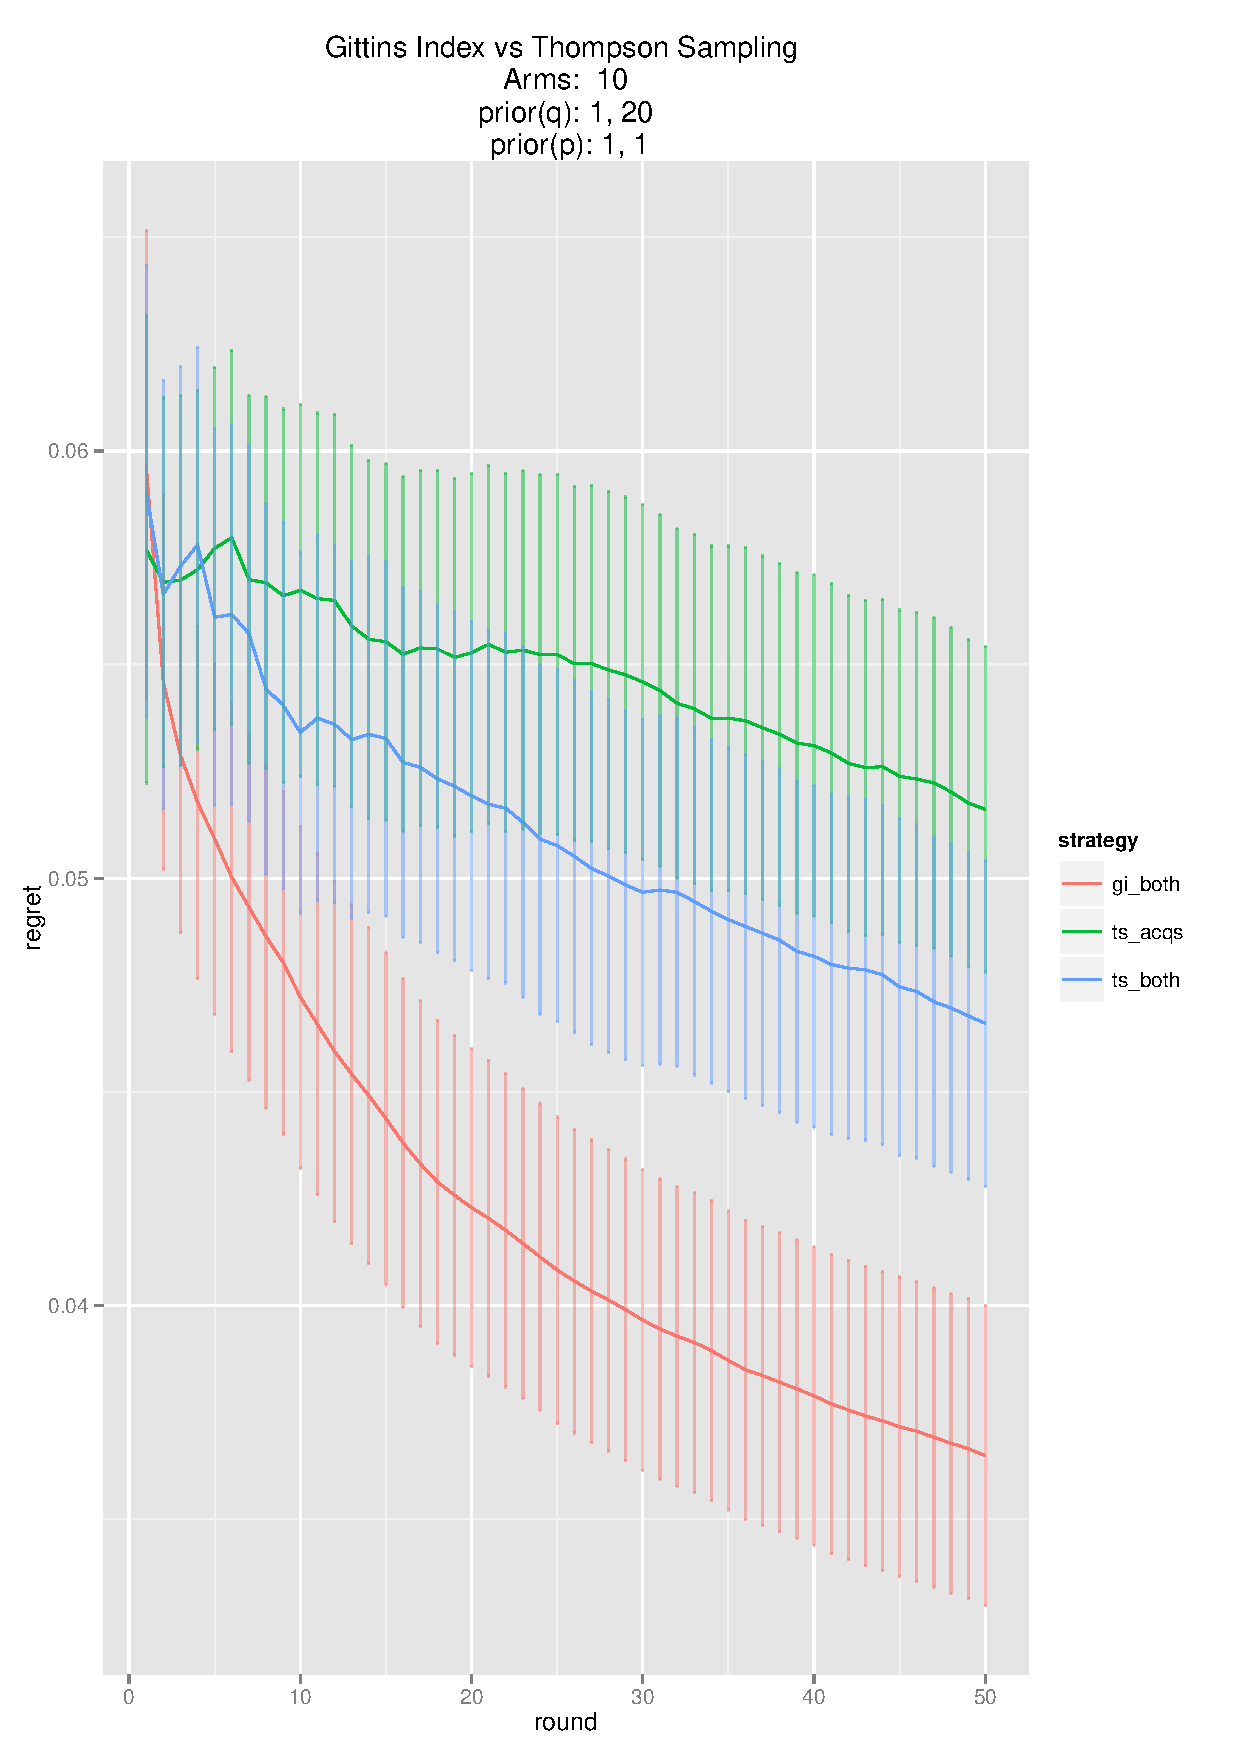
\includegraphics[scale=0.7]{GIBoth.pdf}
    \caption{ Gittins Index vs Thompson Sampling - clicks and acquisitions }
    % \label{fig:GIvsUCB1}
\end{figure}




\chapter{Extensions}

\section{Applicability to other models}

Our decision policy experiments assumed m2 as the underlying model, but our intention here is to provide a template for many different models. 

Both m3 and m5 require more involved sampling techniques to generate samples from their posterior distributions. But Thompson Sampling only requires a single sample point from each arm per round, so for most applications this is perfectly feasible.

We may also possible to apply the GI solution to m3 and m5 models, though taking expectations can only be achieved with Monte Carlo methods, so will be slower.

\section{Contextual bandits}

Factorial bandits are way to bring in regressor information. Here, the rate parameter $p$ is predicted by a probit regression model. The coefficient vector $\mathbf{\theta}$ of the model typically has a multivariate normal prior, which is then updated in a Bayesian fashion. As with our hierarchical models m3 and m5, the posterior does not have an analytic form ~\cite{scott2010modern} but there exist reasonably efficient sampling algorithms for a Thompson Sampling decision policy.

\begin{align}
	c_i \sim Bin(p_i,n_i) \\
	p_i = \Phi(\mathbf{\theta}_i^T \mathbf{x}) \\
	\pi(\mathbf{\theta}_i) = \mathcal{N}(\mu,\Sigma)
\end{align}

Factorial bandits offers a way to bring in important information such as time of day, site and campaign attributes without creating (exponentially many) new arms for every combination. In that sense, it helps us generalise. The same idea can be applied to extend our 2 stage, or even multi-stage model:

\begin{align}
	a_i \sim Bin(q_i,n_i) \\
	c_i \sim Bin(p_i,n_i) \\
	q_i = \Phi(\mathbf{\theta}_i^T \mathbf{x}) \\
	p_i = \Phi(\mathbf{\phi}_i^T \mathbf{x}) \\
	\pi(\mathbf{\theta}_i) = \mathcal{N}(\mu_q,\Sigma_q) \\
	\pi(\mathbf{\phi}_i) = \mathcal{N}(\mu_p,\Sigma_p) 
\end{align}

With m3, $\mu$ and $\Sigma$ would be variables shared across arms and updated online. With m2 they would be updated independently.

As with our earlier models, a well motivated, informative prior on $q_i$ is likely to provide significant performance improvement.

The popular 'contextual bandits' is the name given to factorial bandits, when the features are website viewer information. For example, rather than a site having a single acquisition rate, contextual bandits lets us learn a different reward distribution for different types of user.

\section{Restless bandits}

Restless or non-stationary bandits extend the problem by letting our reward $p$ be a stochastic process, which may jump or drift over time. In effect this introduces an additional filtering problem, though it is rarely explicitly addressed as such.

This can be an important consideration in RTB problems, for example we may see the CTR of a site deteriorate as a campaign becomes over exposed to the site's users. This would have a very detrimental effect on the algorithm's effectiveness.

Discounted UCB ~\cite{garivier2008upper} strategies as well as Dynamic Thompson Sampling ~\cite{gupta2011thompson} address the problem by effectively applying an exponentially weighted moving average filter. 

Consistent with the rest of our work, we suggest there are performance improvements to be made from modelling the specific nature of the non-stationary process, then developing a decision policy based on the model. Although not in general optimal for the restless bandit problem, index strategies can still perform very well. 

We note that although the model is complex, the number of possible outcomes is still the same and so the Gittins index solution has the same order of cost (see Appendix).

\section{Scaling up}

We may extend the $r$ round, 2-stage (clicks an acquisitions) model to $s$ stages. Using Gittins index, we will have $r^s$ states in the final round, meaning we will have an $r^s$ by L matrix, which we perform $r$ matrix multiplications.

There are several ways to reduce the computational cost due to the number of arms - grouping similar arms (e.g. contextual / factorial bandits ) or reuse of similar GI calculations. But the limiting issue is the cost due to large number of rounds.

Given that we are often working with very small rates, we might calculate GI by grouping the updates and enumerating only the more likely outcomes. For example, with a rate of 0.5\%, we might group by 1000 rounds and consider outcomes 0 to 12 which covers 0.998 of the distribution. 
















\cleardoublepage
\phantomsection
% \addcontentsline{toc}{chapter}{\bibname} % Add an entry for the Bibliography in the Table of Contents
%\pagestyle{headings}
% \bibliographystyle{abbrvnat} % set the bibliography style
% \bibliography{bibtexfile} % generate the bibliography
%\bibliographystyle{abbrvnat} % <- Mistake in earlier version. After the bibliography is created it's too late to change the style.
% Pick a sensible bibliography style. 
% If like above you choose to use author-year style citations, you must choose a natbib-compatible bibliographystyle such as 'plainnat'. Abbrvnat is one of the few built-in styles of this type. % You may find many more bibliography styles (*.bst files) online. You can also choose to write your bibliography manually instead of using BibTeX (This will take you longer, unless you plan to use the content of a BibTeX-generated *.bbl file as your starting point).
% When creating a BibTeX file using e.g. reference manager software, note that the entries may contain additional unwanted fields which you would then need to erase. For example, you probably don't want to include the URL of a journal paper in your bibliography.




\bibliography{refs}{}
\bibliographystyle{plain}

%\cleardoublepage \fancyhead[L]{APPENDIX}
\appendix % This line declares that you are starting the appendix.
% If you want a single Appendix and want it to be called Appendix instead of Appendix A, the following should work:
%\setcounter{secnumdepth}{-1} %This turns off automatic chapter numbering
%\chapter{Appendix}


\chapter{Appendix}

\section{Do Clicks Matter}

\subsection{Distribution of a conditioned on n}

Firstly note that:

\begin{align}
{w+a \choose w}{n \choose w+a} &= \frac{n!}{(n-w-a)!w!a} \\
	&= \frac{n!(n-a)!}{((n-a)-w)!w!a!(n-a)!} \\
	&=  {n \choose a}{n-a \choose w}
\end{align}

We may construct the probability mass function for a using the conditional distributions:

\begin{align}
p(a|p,q,n) &= \sum_C p(a|q,c)p(c|p,n) \\
 &= \sum_{c=a}^n {c \choose a} p^a(1-p)^{c-a} {n \choose c} q^c (1-q)^{n-c}
\end{align}

Try to pull out a binomial by reparameterising with $ w = c-a$:

\begin{align}
&= \sum_{w=0}^{n-a} {w+a \choose a} p^a(1-p)^w {n \choose w+a} q^{w+a} (1-q)^{n-w+a} \\
&= {n \choose a} (pq)^a \sum_{c=a}^n {n-a \choose w} ((1-p)q)^w (1-q)^{(n-a)-w} \\
&= {n \choose a} (pq)^a ((1-p)q +  (1-q))^{n-a} \\
&= Binom(a;pq,n)
\end{align}

Ref: http://math.stackexchange.com/questions/626457/conditional-binomials

\subsection{Posterior of qp}

We have now established that a is distributed as $Bin(qp,v)$. The question remains whether the uncertainty around the parameterisation qp is reduced by modelling q and p separately.

For given a,c,n counts, p and q are independent of each other. If we assume a Haldane prior $\beta(0,0)$, we therefore describe their joint density as:

\begin{align}
 f_{P,Q}(p,q|a,c,n) = Beta(p;c,n-c) Beta(q;a,c-a)
\end{align}

Using the same approach as 'Rao, Linear Statistical Inference and its Applications, 3a.3, pg 168' to get the density of pq, apply the following transformation:
\begin{align}
 u(p,q) = qp, \quad v(p,q) = q  \\
 \implies p(u,v) = \frac{u}{v}, \quad q(u,v) = v
\end{align}

\begin{align}
 f_{U,V}(u,v) &= f_{P,Q}(p(u,v),q(u,v)) 
		\frac{\partial p \partial q}{\partial u \partial v} 
		\text{ ,in range }  (u<v<1,0<u<1) \\
 &= Beta(v;c,n-c) Beta(\frac{u}{v};a,c-a) v^{-1} \\
 &= k . v^{c-1} (1-v)^{n-c-1} (\frac{u}{v})^{a-1} (\frac{v - u}{v})^{c-a-1} v^{-1} \\
 &= k . (1-v)^{n-c-1} u^{a-1} (v - u)^{c-a-1}
\end{align}

Now integrate out v. Noting that the integral has the form of a Beta function, we shift and scale the integral with a change of variable.

\begin{align}
\text{Choose }  w &= \frac{v-u}{1-u} \\
f_U(u) &= k.u^{a-1} \int_u^1 (1-v)^{n-c-1} (v - u)^{c-a-1} \mathrm{d}v \\
 &= k.u^{a-1} \int_0^1 ((1-w)(1-u))^{n-c-1} (w(1-u))^{c-a-1} (1-u) \mathrm{d}w \\
 &= k.u^{a-1} (1-u)^{n-a-1} B(n-c,c-a) \\
 &= Beta(u;a,n-a) = Beta(qp;a,n-a) 
\end{align}

Thus showing that under the Haldane prior, click count does not change our estimation. By induction this can be extended to the product of any number of beta variables with appropriate parameters.

\subsection{Posterior of qp - with priors}

We now consider the form of the posterior under different possible priors:

\begin{align}
 f_{P,Q}(p,q|a,c,n) = Beta(p;c+\alpha_p,n-c+\beta_p) Beta(q;a+\alpha_q,c-a+\beta_q)
\end{align}

We can follow the calculation through to step (44) where the $v$ terms no longer cancel out:

\begin{align}
 k . v^{\alpha_p - \alpha_q - \beta_q}(1-v)^{n-c+\beta_p-1} u^{a+\alpha_q-1} (v - u)^{c-a+\beta_q-1}
\end{align}

We see that when $ \alpha_p = \alpha_q + \beta_q $ we will get a Beta form, but otherwise it is not analytic. 

\section{Bayed Adaptive MDP}

We show the Bayes Adaptive MDP for a 2 arm, 2 round game under the 'both' model. Each state, S, is defined by the 8-tuple of prior parameters, updated according to the outcome of each trial. From each state, we have the same control options - arm1 or arm2. There are three possible state transitions - no click, click but no acquisition, click and acquisition. The transition probabilities are the expectations, given the prior values. There is a payoff of 1 for transitions with an acquisition.

\begin{align}
s0 =
 \begin{pmatrix}
  \alpha_{p,1} & \beta_{p,1} & \alpha_{q,1} & \beta_{q,1} \\
  \alpha_{p,2} & \beta_{p,2} & \alpha_{q,2} & \beta_{q,2} 
 \end{pmatrix} \\
s1 =
  \begin{pmatrix}
   \alpha_{p,1}+1 & \beta_{p,1} & \alpha_{q,1}+1 & \beta_{q,1} \\
   \alpha_{p,2} & \beta_{p,2} & \alpha_{q,2} & \beta_{q,2} 
  \end{pmatrix} \\
s2 =
  \begin{pmatrix}
   \alpha_{p,1} & \beta_{p,1}+1 & \alpha_{q,1}+1 & \beta_{q,1} \\
   \alpha_{p,2} & \beta_{p,2} & \alpha_{q,2} & \beta_{q,2} 
  \end{pmatrix} \\
\vdots \\
s6 =
  \begin{pmatrix}
   \alpha_{p,1} & \beta_{p,1} & \alpha_{q,1} & \beta_{q,1} \\
   \alpha_{p,2} & \beta_{p,2} & \alpha_{q,2} & \beta_{q,2}+1 
  \end{pmatrix}
\end{align} 

\begin{figure}[p]
    \centering
    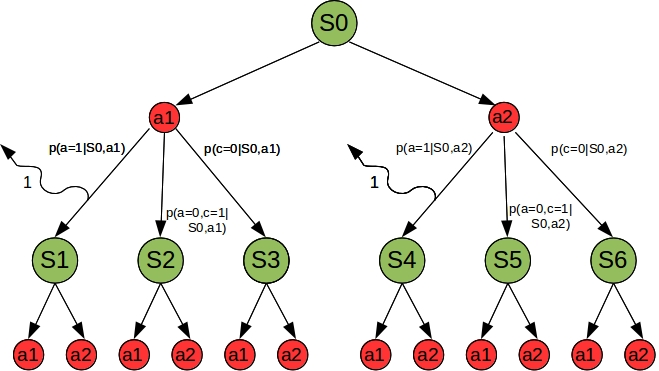
\includegraphics[scale=0.6]{BAMDP.jpg}
    \caption{ Bayes Adaptive Markov Decision Process - Model 2 }
    % \label{fig:GIvsUCB1}
\end{figure}


Note that although the posterior of pq does not have a closed form, it is still a cheap operation to take the expectation due to the independence of p and q. This means the both model is of similar order cost to the clicks-only or acquisitions-only model.

\begin{align}
	p(a=1|S,a1) = E[qp] = E[q]E[p] = 
		\left( \frac{ \alpha_{q,1} }{ \alpha_{q,1} + \beta_{q,1} } \right)
		\left( \frac{ \alpha_{p,1} }{ \alpha_{p,1} + \beta_{p,1} } \right) \\
	p(a=0,c=1|S,a1) = 
		\left( \frac{ \beta_{q,1} }{ \alpha_{q,1} + \beta_{q,1} } \right)
		\left( \frac{ \alpha_{p,1} }{ \alpha_{p,1} + \beta_{p,1} } \right) \\
	p(c=0|S,a1) = 
		\left( \frac{ \beta_{p,1} }{ \alpha_{p,1} + \beta_{p,1} } \right) 
\end{align}	

The optimal policy under this MDP is to greedily choose action with maximum value. The value for each of the 12 actions in the second round is simply the expected payoff $E[qp]$ given the state S1-S6 that the action is being taken from. The value of actions in the first round is the expectation of their immediate payoff, plus the expectation of the maximum value in the second round.

\section{Gittins index calculation}

We can adapt the above MDP to calculate a Gittins index for arm 1. To do this, we replace arm 2 with an arm with fixed payoff $\lambda$. We may then calculate the maximum possible payoff of arm 2 such that both arms have equal value in the first round. The most efficient method to do this is the 'calibration method' whereby a matrix of 'candidate' $\lambda$ values is used to calculate the index to arbitrary precision.

To adapt the calibration algorithm described in Nino-Mora ~\cite{nino2011computing} to our 2 stage binomial model, we need to develop a schema for constructing transition matrices for information states between rounds.

Each information state can be represented as a tuple $(c,a)$. If we sort the information states by clicks followed by acquisitions, we can assign each state to a contiguous range of indices, such that:

\begin{align}
	\operatorname{index}(c,a) = 1 + \sum_j^c + a = 1 + a + \frac{c + c^2}{2} 
\end{align}

At each round $t$, we construct an $i$ by $j$ transition matrix $P_t$. For each information state $i$, we populate the transition probabilities for the 3 outcomes:

No clicks keeps same index:
\begin{align}
	&P(i,i) = 1 - E[p|c,a]
\end{align}

Click but no acquisition advances index by c+1:
\begin{align}
	&P(i,i+c+1) = (1 - E[q|c,a])E[p|c,a] 
\end{align}

Click and acquisition advances index by c+1+1:
\begin{align}
	&P(i,i+c+2) = E[q|c,a]E[p|c,a] 
\end{align}

At this point we have not specified the nature of the model. In fact, the algorithm is identical for all 2 stage binomial models. The only thing we need from the model are the conditional expectations for the information state transitions. Like Thompson Sampling, this orthogonality is very attractive from an implementation point of view.

For the M2 model used in our experiments, the expectations are:
\begin{align}
	E[p|c,a] = \frac{\alpha_p + c}{\alpha_p + \beta_p + t} \\
	E[q|c,a] = \frac{\alpha_q + a}{\alpha_q + \beta_q + c}
\end{align}

So, for example, $P_1$, assuming flat priors would look like the following:

\begin{align}
P_1 =
\begin{pmatrix}
  2\mathbin{/}3 & 1\mathbin{/}6 & 1\mathbin{/}6 & 0 & 0 & 0\\
  0 & 1\mathbin{/}3 & 0 & 4\mathbin{/}9 & 2\mathbin{/}9 & 0\\
  0 & 0 & 1\mathbin{/}3 & 0 & 2\mathbin{/}9 & 4\mathbin{/}9\\
\end{pmatrix}
\end{align}


Note - $P_t$ is a very sparse matrix, one should use a sparse matrix implementation for large space and speed performance improvements.

\end{document}
